%! BibTeX Compiler = bibtex
%DIF LATEXDIFF DIFFERENCE FILE
%DIF DEL main-revision.tex   Wed Mar 13 15:41:30 2024
%DIF ADD main.tex            Fri Jun 14 16:20:18 2024
%TC:ignore
\documentclass{article}
\usepackage{caption}
\usepackage{censor}
\usepackage{xcolor, colortbl}
\definecolor{BLUELINK}{HTML}{0645AD}
\definecolor{DARKBLUELINK}{HTML}{0B0080}
\definecolor{LIGHTGREY}{gray}{0.9}
\PassOptionsToPackage{hyphens}{url}
\usepackage[colorlinks=false]{hyperref}
% for linking between references, figures, TOC, etc in the pdf document
\hypersetup{colorlinks,
    linkcolor=DARKBLUELINK,
    anchorcolor=DARKBLUELINK,
    citecolor=DARKBLUELINK,
    filecolor=DARKBLUELINK,
    menucolor=DARKBLUELINK,
    urlcolor=BLUELINK
} % Color citation links in purple
\PassOptionsToPackage{unicode}{hyperref}
\PassOptionsToPackage{naturalnames}{hyperref}

\usepackage{biorxiv}

\usepackage{url}
\usepackage{amssymb,amsfonts,amsmath,amsthm,mathtools}
\usepackage{lmodern}
\usepackage{xfrac, nicefrac}
\usepackage{bm}
\usepackage{listings, enumerate, enumitem}
\usepackage[export]{adjustbox}
\usepackage{graphicx}
\usepackage{bbold}
\usepackage{pdfpages}
\pdfinclusioncopyfonts=1
\usepackage{lineno}
\usepackage{tabu}
\usepackage{hhline}
\usepackage{multicol,multirow,array}
\usepackage{etoolbox}
\usepackage{booktabs}
\usepackage{makecell}
\usepackage{marvosym}

% -- Defining colors:
\definecolor{backcolour}{rgb}{0.95,0.95,0.92}% Definig a custom style:
\lstdefinestyle{mystyle}{
    backgroundcolor=\color{backcolour},
    basicstyle=\ttfamily\scriptsize\bfseries,
    breakatwhitespace=false,
    breaklines=true,
    captionpos=t,
    keepspaces=true,
    showspaces=false,
    showstringspaces=false,
    showtabs=false,
    tabsize=2
}% -- Setting up the custom style:
\lstset{style=mystyle}
\captionsetup[table]{hypcap=false}
\captionsetup[figure]{hypcap=false}

\newcommand{\defEqual}{\stackrel{\text{def}}{=}}
\newcommand{\Multiply}{\cdot}
\newcommand{\MultiplyMatrix}{\times}
\newcommand{\UniDimArray}[1]{\bm{#1}}
\newcommand{\BiDimArray}[1]{\bm{#1}}
\newcommand{\tr}{^{\intercal}}
\newcommand{\inv}{^{-1}}
\DeclareMathOperator{\E}{\mathbb{E}}
\DeclareMathOperator{\Var}{\text{var}}
\DeclareMathOperator{\Cov}{\text{cov}}
\newcommand{\Qst}{Q$_\text{ST}$}
\newcommand{\Fst}{F$_\text{ST}$}
\newcommand{\QstFst}{\Qst--\Fst}
\newcommand{\der}{\mathrm{d}}
\newcommand{\e}{\text{e}}
\newcommand{\Ne}{N_{\text{e}}}
\newcommand{\dnds}{\omega}
\newcommand{\pn}{\pi_N}
\newcommand{\ps}{\pi_S}
\newcommand{\pnps}{\pn / \ps}
\newcommand{\proba}{\mathbb{P}}
\newcommand{\pfix}{\proba_{\text{fix}}}
\newcommand{\Indiv}{k}
\newcommand{\Branch}{b}
\newcommand{\WishartIDD}{m}
\newcommand{\Spi}{i}
\newcommand{\Spj}{j}
\newcommand{\NbrTaxa}{n}
\newcommand{\Time}{t}
\newcommand{\NbrGen}{t_{\Spi, \Spj}}
\newcommand{\NucDiv}{d_{\Spi, \Spj}}
\newcommand{\Trait}{P}
\newcommand{\Heritability}{h^2}
\newcommand{\HeritabilitySpi}{\Heritability_{\Spi}}
\newcommand{\MeanTrait}{\bar{\Trait}}
\newcommand{\VecTrait}{\UniDimArray{\bar{\Trait}}}
\newcommand{\RootTrait}{\phi}
\newcommand{\VarPhy}{\Cov \left( \MeanTrait_{\Spi}, \MeanTrait_{\Spj}\right)}
\newcommand{\VecZero}{\UniDimArray{0}}
\newcommand{\VecOne}{\UniDimArray{1}}
\newcommand{\Distance}{\BiDimArray{D}}
\newcommand{\DistanceMatrix}{\BiDimArray{\Distance}}
\newcommand{\MutationRatePheno}{\mu}
\newcommand{\MutationRateNuc}{u}
\newcommand{\SubRate}{q}
\newcommand{\NbrLoci}{L}
\newcommand{\VarPhenotype}{V_{\Trait}}
\newcommand{\VarPhenotypeSpi}{V_{\Trait, \Spi}}
\newcommand{\VarGenetic}{V_{\mathrm{A}}}
\newcommand{\VarGeneticSpi}{V_{\mathrm{A}, \Spi}}
\newcommand{\VarEnv}{V_{\mathrm{E}}}
\newcommand{\VarMutation}{V_{\mathrm{M}}}
\newcommand{\GenArchi}{\NbrLoci \Multiply \E \left[ a^2 \right]}
\newcommand{\RateMut}{\sigma^2_{\mathrm{M}}}
\newcommand{\RateBetween}{\sigma^2_{\mathrm{B}}}
\newcommand{\RateWhithin}{\sigma^2_{\mathrm{W}}}
\newcommand{\RateWhithinSpi}{\sigma^2_{\mathrm{W}, \Spi}}
\newcommand{\VecRateWhithin}{\UniDimArray{\RateWhithin}}
\newcommand{\EstRateBetween}{\widehat{\sigma}^2_{\mathrm{B}}}
\newcommand{\EstRateWhithin}{\widehat{\sigma}^2_{\mathrm{W}}}
\newcommand{\NI}{\rho}
\newcommand{\EstNI}{\widehat{\rho}}
\newcommand{\StdSelection}{\sigma}
\newcommand{\VarSelection}{\StdSelection^2}

% Tree
\newcommand{\Nbranch}{2 \NbrTaxa - 2}
\newcommand{\WishartPostDf}{2 \NbrTaxa + 1}
\newcommand{\Ntrait}{K}
\newcommand{\contrast}{\UniDimArray{C}}
\newcommand{\Covariancematrix}{\Sigma}
\newcommand{\CovarianceMatrix}{\BiDimArray{\Covariancematrix}}
\newcommand{\Precisionmatrix}{\Omega}
\newcommand{\PrecisionMatrix}{\BiDimArray{\Precisionmatrix}}
\newcommand{\Identitymatrix}{\BiDimArray{I}}
\newcommand{\brownian}{\mathcal{B}}
\newcommand{\Brownian}{\UniDimArray{\brownian}}
\newcommand{\Scattermatrix}{\BiDimArray{A}}
\newcommand{\Multivariate}{\UniDimArray{Z}}

\renewcommand{\baselinestretch}{1.5}
\renewcommand{\arraystretch}{1.2}
\linenumbers
\frenchspacing

\title{Detecting diversifying selection for a trait from within and between-species genotypes and phenotypes}
\rhead{\scshape Trait selection from within and between-species variation}

\author{~}
%DIF PREAMBLE EXTENSION ADDED BY LATEXDIFF
%DIF UNDERLINE PREAMBLE %DIF PREAMBLE
\RequirePackage[normalem]{ulem} %DIF PREAMBLE
\RequirePackage{color}\definecolor{RED}{rgb}{1,0,0}\definecolor{BLUE}{rgb}{0,0,1} %DIF PREAMBLE
\providecommand{\DIFaddtex}[1]{{\protect\color{blue}\uwave{#1}}} %DIF PREAMBLE
\providecommand{\DIFdeltex}[1]{{\protect\color{red}\sout{#1}}}                      %DIF PREAMBLE
%DIF SAFE PREAMBLE %DIF PREAMBLE
\providecommand{\DIFaddbegin}{} %DIF PREAMBLE
\providecommand{\DIFaddend}{} %DIF PREAMBLE
\providecommand{\DIFdelbegin}{} %DIF PREAMBLE
\providecommand{\DIFdelend}{} %DIF PREAMBLE
\providecommand{\DIFmodbegin}{} %DIF PREAMBLE
\providecommand{\DIFmodend}{} %DIF PREAMBLE
%DIF FLOATSAFE PREAMBLE %DIF PREAMBLE
\providecommand{\DIFaddFL}[1]{\DIFadd{#1}} %DIF PREAMBLE
\providecommand{\DIFdelFL}[1]{\DIFdel{#1}} %DIF PREAMBLE
\providecommand{\DIFaddbeginFL}{} %DIF PREAMBLE
\providecommand{\DIFaddendFL}{} %DIF PREAMBLE
\providecommand{\DIFdelbeginFL}{} %DIF PREAMBLE
\providecommand{\DIFdelendFL}{} %DIF PREAMBLE
%DIF HYPERREF PREAMBLE %DIF PREAMBLE
\providecommand{\DIFadd}[1]{\texorpdfstring{\DIFaddtex{#1}}{#1}} %DIF PREAMBLE
\providecommand{\DIFdel}[1]{\texorpdfstring{\DIFdeltex{#1}}{}} %DIF PREAMBLE
\newcommand{\DIFscaledelfig}{0.5}
%DIF HIGHLIGHTGRAPHICS PREAMBLE %DIF PREAMBLE
\RequirePackage{settobox} %DIF PREAMBLE
\RequirePackage{letltxmacro} %DIF PREAMBLE
\newsavebox{\DIFdelgraphicsbox} %DIF PREAMBLE
\newlength{\DIFdelgraphicswidth} %DIF PREAMBLE
\newlength{\DIFdelgraphicsheight} %DIF PREAMBLE
% store original definition of \includegraphics %DIF PREAMBLE
\LetLtxMacro{\DIFOincludegraphics}{\includegraphics} %DIF PREAMBLE
\newcommand{\DIFaddincludegraphics}[2][]{{\color{blue}\fbox{\DIFOincludegraphics[#1]{#2}}}} %DIF PREAMBLE
\newcommand{\DIFdelincludegraphics}[2][]{% %DIF PREAMBLE
\sbox{\DIFdelgraphicsbox}{\DIFOincludegraphics[#1]{#2}}% %DIF PREAMBLE
\settoboxwidth{\DIFdelgraphicswidth}{\DIFdelgraphicsbox} %DIF PREAMBLE
\settoboxtotalheight{\DIFdelgraphicsheight}{\DIFdelgraphicsbox} %DIF PREAMBLE
\scalebox{\DIFscaledelfig}{% %DIF PREAMBLE
\parbox[b]{\DIFdelgraphicswidth}{\usebox{\DIFdelgraphicsbox}\\[-\baselineskip] \rule{\DIFdelgraphicswidth}{0em}}\llap{\resizebox{\DIFdelgraphicswidth}{\DIFdelgraphicsheight}{% %DIF PREAMBLE
\setlength{\unitlength}{\DIFdelgraphicswidth}% %DIF PREAMBLE
\begin{picture}(1,1)% %DIF PREAMBLE
\thicklines\linethickness{2pt} %DIF PREAMBLE
{\color[rgb]{1,0,0}\put(0,0){\framebox(1,1){}}}% %DIF PREAMBLE
{\color[rgb]{1,0,0}\put(0,0){\line( 1,1){1}}}% %DIF PREAMBLE
{\color[rgb]{1,0,0}\put(0,1){\line(1,-1){1}}}% %DIF PREAMBLE
\end{picture}% %DIF PREAMBLE
}\hspace*{3pt}}} %DIF PREAMBLE
} %DIF PREAMBLE
\LetLtxMacro{\DIFOaddbegin}{\DIFaddbegin} %DIF PREAMBLE
\LetLtxMacro{\DIFOaddend}{\DIFaddend} %DIF PREAMBLE
\LetLtxMacro{\DIFOdelbegin}{\DIFdelbegin} %DIF PREAMBLE
\LetLtxMacro{\DIFOdelend}{\DIFdelend} %DIF PREAMBLE
\DeclareRobustCommand{\DIFaddbegin}{\DIFOaddbegin \let\includegraphics\DIFaddincludegraphics} %DIF PREAMBLE
\DeclareRobustCommand{\DIFaddend}{\DIFOaddend \let\includegraphics\DIFOincludegraphics} %DIF PREAMBLE
\DeclareRobustCommand{\DIFdelbegin}{\DIFOdelbegin \let\includegraphics\DIFdelincludegraphics} %DIF PREAMBLE
\DeclareRobustCommand{\DIFdelend}{\DIFOaddend \let\includegraphics\DIFOincludegraphics} %DIF PREAMBLE
\LetLtxMacro{\DIFOaddbeginFL}{\DIFaddbeginFL} %DIF PREAMBLE
\LetLtxMacro{\DIFOaddendFL}{\DIFaddendFL} %DIF PREAMBLE
\LetLtxMacro{\DIFOdelbeginFL}{\DIFdelbeginFL} %DIF PREAMBLE
\LetLtxMacro{\DIFOdelendFL}{\DIFdelendFL} %DIF PREAMBLE
\DeclareRobustCommand{\DIFaddbeginFL}{\DIFOaddbeginFL \let\includegraphics\DIFaddincludegraphics} %DIF PREAMBLE
\DeclareRobustCommand{\DIFaddendFL}{\DIFOaddendFL \let\includegraphics\DIFOincludegraphics} %DIF PREAMBLE
\DeclareRobustCommand{\DIFdelbeginFL}{\DIFOdelbeginFL \let\includegraphics\DIFdelincludegraphics} %DIF PREAMBLE
\DeclareRobustCommand{\DIFdelendFL}{\DIFOaddendFL \let\includegraphics\DIFOincludegraphics} %DIF PREAMBLE
%DIF COLORLISTINGS PREAMBLE %DIF PREAMBLE
\RequirePackage{listings} %DIF PREAMBLE
\RequirePackage{color} %DIF PREAMBLE
\lstdefinelanguage{DIFcode}{ %DIF PREAMBLE
%DIF DIFCODE_UNDERLINE %DIF PREAMBLE
  moredelim=[il][\color{red}\sout]{\%DIF\ <\ }, %DIF PREAMBLE
  moredelim=[il][\color{blue}\uwave]{\%DIF\ >\ } %DIF PREAMBLE
} %DIF PREAMBLE
\lstdefinestyle{DIFverbatimstyle}{ %DIF PREAMBLE
	language=DIFcode, %DIF PREAMBLE
	basicstyle=\ttfamily, %DIF PREAMBLE
	columns=fullflexible, %DIF PREAMBLE
	keepspaces=true %DIF PREAMBLE
} %DIF PREAMBLE
\lstnewenvironment{DIFverbatim}{\lstset{style=DIFverbatimstyle}}{} %DIF PREAMBLE
\lstnewenvironment{DIFverbatim*}{\lstset{style=DIFverbatimstyle,showspaces=true}}{} %DIF PREAMBLE
%DIF END PREAMBLE EXTENSION ADDED BY LATEXDIFF

\begin{document}

\maketitle

% Abstract (≤ 250 words)
%TC:endignore
\begin{abstract}
    To quantify selection acting on a trait, methods have been developed using either within or between-species variation.
    However, methods using within-species variation do not integrate the changes at the macro-evolutionary scale.
    Conversely, current methods using between-species variation usually discard within-species variation, thus not accounting for processes at the micro-evolutionary scale.
    The main goal of this study is to define a neutrality index for a quantitative trait, by combining within- and between-species variation.
    This neutrality index integrates nucleotide polymorphism and divergence for normalizing trait variation.
    As such, it does not require estimation of population size nor of time of speciation for normalization.
    Our index can be used to seek deviation from the null model of neutral evolution, and test for diversifying selection.
    Applied to brain mass and body mass at the mammalian scale, we show that brain mass is under diversifying selection.
    Finally, we show that our test is not sensitive to the assumption that population sizes, mutation rates and generation time are constant across the phylogeny, and automatically adjust for it.
\end{abstract}

\keywords{Quantitative genetics \and Trait evolution \and Selection \and Phylogenetics \and Population genetics }

% Research Article (7500 words)
\section*{Introduction}\label{sec:introduction}

Determining whether a trait is under a particular regime of selection has been a long-standing goal in evolutionary biology.
Fundamentally, distinguishing neutral evolution from selection requires determining which selective regime is supported by the observed variation of traits or sequences.
The variation of phenotypes (traits) and genotypes (sequences) can be observed at different scales, across different development stages at the individual level, across different individuals and populations at the species level, and finally across different species at the phylogenetic level.
All these systems require different assumptions and methodologies, and the endeavor to determine the selective regime for a given trait has thus incorporated theories, methods, and developments across various fields of evolutionary biology such as quantitative genetics, population genetics, phylogenetics and comparative genomics~\citep{lynch_genetics_1998, walsh_evolution_2018}.

Leveraging individual variations within the same species, Genome-Wide Association Studies (GWAS) in humans have shown that traits are mostly polygenic (many loci associated with a given trait) and under stabilizing selection, while the loci affecting those traits are mostly pleiotropic (many traits associated with a given locus) with additive effects~\citep{simons_population_2018, sella_thinking_2019}.
Given this genetic architecture of traits, from two diverging populations, it is possible to distinguish which traits have evolved under natural selection in controlled experimental settings, by performing genetic cross between individuals~\citep{fraser_detecting_2020}.
Across several populations, by contrasting both trait differentiation (\Qst) and genetic differentiation (\Fst), so-called \QstFst\ methods have been used to determine the selective regime and to quantify the strength of selection acting on a trait~\citep{merila_comparison_2001, leinonen_comparative_2008}.
\Qst\ higher than \Fst\ is interpreted as a signature of diversifying selection due to adaptation to different optimum trait values in the different populations.
Contrarily, \Qst\ lower than \Fst\ is interpreted as a signature of stabilizing selection~\citep{lamy_qst_2012}.
Other frameworks explicitly model genetic drift as a random process generating both trait and genetic differences between individuals and populations.
This integrated framework can discriminate between selection and genetic drift as a cause of trait differentiation between populations of the same species~\citep{ovaskainen_new_2011}.
However, regardless of the strengths and weaknesses of each method\DIFaddbegin \DIFadd{~}\DIFaddend \citep{pujol_are_2008, edelaar_comparisons_2011, ovaskainen_new_2011}, tests of trait differentiation between populations are ultimately limited to recent local adaptation since they are based on the variation observed within a single species.

% Pair of species
To disentangle selection from neutral evolution, trait variation can also be observed at a larger time scale.
For example, starting from the same ancestral population, divergent lineages accumulate phenotypic changes that will reach fixation in the population.
These changes ultimately result in different mean trait values across lineages.
Theoretically, the variance in mean trait value (between lineages) does increase linearly with time of divergence, and also proportionally to the trait variance at the population scale~\DIFdelbegin \DIFdel{\mbox{%DIFAUXCMD
\citep{lande_genetic_1980, turelli_heritable_1984}}\hskip0pt%DIFAUXCMD
}\DIFdelend \DIFaddbegin \DIFadd{\mbox{%DIFAUXCMD
\citep{lande_genetic_1980, turelli_heritable_1984, felsenstein_phylogenies_1988a}}\hskip0pt%DIFAUXCMD
}\DIFaddend .
Empirically, this effect can be observed for genes with larger within-species variation in gene expression level, which exhibits a faster accumulation of divergence in mean expression level~\citep{khaitovich_neutral_2004}.
As an analogy, in the context of protein-coding DNA sequences, leveraging within species variation and divergence to a sister species is the crux of the \citet{mcdonald_adaptative_1991} test.
In such a test, inflation of divergence to the sister species is compared to polymorphism within species, while neutral makers (usually synonymous sites) are used to determine the neutral expectation and thus are used for normalization.
Altogether, both the trait variance and the evolution in mean value can be used to test for trait selection in a pair of species~\citep{walsh_evolution_2018}.

% Phylogenetics (mean trait evolution)
Alternatively, by accounting for the underlying relationships between several species, the selective regime for a quantitative trait can also be tested at the phylogenetic scale~\citep{felsenstein_phylogenies_1985}.
Under neutral evolution, the change in mean trait value along a given branch of the tree is normally distributed, with a variance proportional to divergence time~\DIFdelbegin \DIFdel{\mbox{%DIFAUXCMD
\citep{hansen_translating_1996}}\hskip0pt%DIFAUXCMD
}\DIFdelend \DIFaddbegin \DIFadd{\mbox{%DIFAUXCMD
\citep{felsenstein_phylogenies_1985, felsenstein_phylogenies_1988a, hansen_translating_1996}}\hskip0pt%DIFAUXCMD
}\DIFaddend .
As a result, the mean trait value can be modeled as a Brownian process branching at every node of the tree~\citep{hansen_translating_1996, harmon_phylogenetic_2018}.
Reconstructing the trait variation along the whole phylogeny as a Brownian process can thus constitute a null model of neutral trait evolution.
Deviations from the assumptions of the Brownian process are however well known.
When trait variation is constrained because of optimum mean trait values across or between species, the pattern of evolution can be modeled by the Ornstein-Uhlenbeck processes, which is often interpreted as a signature of stabilizing selection~\DIFdelbegin \DIFdel{\mbox{%DIFAUXCMD
\citep{catalan_drift_2019}}\hskip0pt%DIFAUXCMD
}\DIFdelend \DIFaddbegin \DIFadd{\mbox{%DIFAUXCMD
\citep{hansen_stabilizing_1997, catalan_drift_2019}}\hskip0pt%DIFAUXCMD
}\DIFaddend .
Alternatively, a trend in the Brownian process (the tendency of a trait to evolve in a certain direction without fixed optimum) is interpreted as a signature of directional selection at the phylogenetic scale~\citep{silvestro_early_2019}.
However, studies have shown that such comparative approaches are subject to different biases~\citep{harmon_phylogenetic_2018}.
First, a trait under stabilizing selection for which the optimal trait value is also changing as a Brownian process will not deviate from a Brownian process, and thus be wrongly classified as neutral~\citep{hansen_translating_1996}.
In other words, the better fit of a Brownian process does not necessarily constitute proof of the neutral model.
\DIFdelbegin \DIFdel{Also}\DIFdelend \DIFaddbegin \DIFadd{Second}\DIFaddend , a better fit of a Brownian could be due to a trait evolving with a rate \DIFdelbegin \DIFdel{two }\DIFdelend \DIFaddbegin \DIFadd{too }\DIFaddend low compared to the timespan on which it is measured~\citep{grabowski_cautionary_2023}.
\DIFdelbegin \DIFdel{Second}\DIFdelend \DIFaddbegin \DIFadd{And third}\DIFaddend , even for a trait evolving under a neutral regime, the Ornstein-Uhlenbeck process might sometimes be statistically preferred over a Brownian process due to sampling artifacts~\citep{silvestro_measurement_2015, cooper_cautionary_2016, price_detecting_2022}.
Those limitations, altogether with the use of mean trait estimates leaving out the variance in traits between individuals, easily generate misclassification of selection from methods at the phylogenetic scale.

% At the frontier Phylogenetics/Population-genetics
At the frontier between micro and macro-evolution, comparative methods at the phylogenetic scale have acknowledged the importance of modeling within-species variation together with changes in mean trait value to either describe measurement errors~\citep{lynch_methods_1991, hansen_interpreting_2012}, incorporate values for individuals~\citep{felsenstein_comparative_2008} or to scale the rate of change in mean trait value~\citep{kostikova_bridging_2016, gaboriau_multiplatform_2020, gaboriau_exploring_2023}.
\DIFdelbegin \DIFdel{Between to }\DIFdelend \DIFaddbegin \DIFadd{Across many species, }\DIFaddend within-species variation has also been used to infer diversifying selection by estimating the ratio of between to within \DIFaddbegin \DIFadd{species }\DIFaddend variation of many traits and test for deviation from the average ratio across traits~\citep{rohlfs_modeling_2014, rohlfs_phylogenetic_2015}.
Here, our goal was again to use both variances between and within species to determine the selective regime of a quantitative trait.
We build a novel framework that integrates trait variation at the phylogenetic and population scales together with estimates of nucleotide sequence variations at both scales.
It allowed us to define an expected ratio of normalized variance between and within species while setting the threshold of this ratio for neutral, stabilizing, and diversifying selection.
The ratio that we propose can be considered as a neutrality index for \DIFdelbegin \DIFdel{a }\DIFdelend any quantitative trait \DIFaddbegin \DIFadd{~\mbox{%DIFAUXCMD
\citep{lynch_rate_1990}}\hskip0pt%DIFAUXCMD
, while }\DIFaddend articulating trait and nucleotide variation within and between species.
Importantly, our neutrality index also leverages nucleotide divergence and polymorphism to normalize trait variation at both scales, such that it does not require estimating population size (within-species) or speciation time (between species).
From the field of population genetics, while \QstFst\ methods and their derivatives ultimately seek trait differentiation among different populations from the same species~\citep{pujol_are_2008, ovaskainen_new_2011}, our study can be seen as their macro-evolutionary \DIFdelbegin \DIFdel{generalization }\DIFdelend \DIFaddbegin \DIFadd{analog }\DIFaddend to account for phylogenetic relationships between species.
From the field of phylogenetics, our study can be seen as an alternative to the EVE model~\citep{rohlfs_modeling_2014, rohlfs_phylogenetic_2015} for a single trait, where we set a threshold for neutral evolution by leveraging species nucleotide polymorphism and divergence.


\section*{Materials and Methods}\label{sec:materials-and-methods}
\subsection*{Neutrality index for a quantitative trait}\label{subsec:neutrality-index-for-a-quantitative-trait}

While observing trait variations across individuals of several species, we ask if the variation within species compared to variation between species is compatible with neutral evolution or not.
In statistical terms, this can also be framed as: Is the variance of means equal to the mean of variances?
The difficulty in such a study is that individuals are not independent samples, but are from species that diverged at different times.
By reviewing theoretical expectations and leveraging nucleotide sequence variations, the goal of this section is thus to obtain normalized trait variation between and within species that are equal if the trait is neutral.
Here we denote these normalized trait variations as respectively $\RateWhithin$ for within species and as $\RateBetween$ for between species.

\subsubsection*{Within-species trait variations}

For a given trait, the genetic architecture is mainly defined by the number of loci encoding the trait ($\NbrLoci$) and the random additive effect of a mutation on the trait ($a$).
For a diploid individual, the mutational variance ($\VarMutation$) is the rate at which new mutations contribute to the trait variance per generation.
As shown in \citet{lande_quantitative_1979, lande_sexual_1980}, $\VarMutation$ is a function of the mutation rate per locus per generation ($\MutationRatePheno$) and the genetic architecture of the trait as:
\begin{gather}
    \VarMutation = 2 \MutationRatePheno \Multiply \GenArchi \label{eq:var-mutation}.
\end{gather}

While in an infinitesimal model mutations supply new genetic variants, random genetic drift depletes standing variation~\citep{turelli_commentary_2017, barton_infinitesimal_2017, sella_thinking_2019}.
For a neutral trait at equilibrium between mutation and drift~\citep{lynch_mutation_1998}, the additive genetic variance in a species ($\VarGenetic$) is a function of the mutational variance ($\VarMutation$) and the effective number of individuals in the population ($\Ne$):
\begin{align}
    \VarGenetic & =  2 \Ne \Multiply \VarMutation, \\
    & = 4 \Ne \Multiply \MutationRatePheno \Multiply \GenArchi \text{ from eq.~\ref{eq:var-mutation}}\label{eq:var-genetic}.
\end{align}

For any neutral genomic region of interest, the nucleotide diversity, $\pi$, is the average number of differences between pairs of sequences drawn at random, which is also equal to the sum of expected heterozygosities over all nucleotide sites~\citep{tajima_statistical_1989}.
Any segregating mutations will eventually reach fixation or extinction due to random genetic drift and $\pi$ is also at a balance between mutations and drift.
As shown in \citet{tajima_statistical_1989}, $\pi$ is a function of the mutation rate ($\MutationRateNuc$, per nucleotide site per generation) and the effective population size ($\Ne$):
\begin{gather}
    \pi = 4 \Ne \Multiply \MutationRateNuc \label{eq:genetic-diversity}.
\end{gather}

To remove the effect of $\Ne$, we define $\RateWhithin$ as the ratio of additive genetic variance of the trait ($\VarGenetic$) over $\pi$ of any neutral genomic region of interest.
After simplification, $\RateWhithin$ is then solely a function of the underlying genetic architecture as:
\begin{align}
    \RateWhithin & \defEqual \frac{\VarGenetic }{\pi} \label{eq:def-rate-pop}, \\
    & = \frac{4 \Ne \Multiply \MutationRatePheno \Multiply \GenArchi}{4 \Ne \Multiply \MutationRateNuc} \text{ from eq.~\ref{eq:var-mutation} and~\ref{eq:genetic-diversity}}, \\
    & = \frac{\MutationRatePheno \Multiply \GenArchi}{\MutationRateNuc}. \label{eq:rate-pop}
\end{align}

If $\VarGenetic$ is not empirically accessible, it can be related to the observed phenotypic variance ($\VarPhenotype$), multiplied by narrow-sense heritability of the trait ($\Heritability$), as~\citep{hill_data_2008}:
\begin{align}
    \VarGenetic & = \Heritability \Multiply \VarPhenotype.\label{eq:var-gen-pheno}
\end{align}
Which leads to $\RateWhithin$ being a function of $\VarPhenotype$ and $\Heritability$ instead of $\VarGenetic$ as:
\begin{align}
    \RateWhithin & = \frac{\Heritability \Multiply \VarPhenotype }{\pi } \text{ from definition eq.~\ref{eq:def-rate-pop} and~\ref{eq:var-gen-pheno}}, \label{eq:def-rate-pheno-pop} \\
    & = \frac{\MutationRatePheno \Multiply \GenArchi}{\MutationRateNuc} \text{ from eq.~\ref{eq:rate-pop}} \label{eq:rate-pheno-pop}
\end{align}

\subsubsection*{Between-species trait variations}\label{subsec:between-species-var}
For a given species $\Spi$, we denote by $\MeanTrait_{\Spi}$ the mean value of the trait across the individuals.
If the trait is neutral and encoded by many loci as assumed by the infinitesimal model, $\MeanTrait_{\Spi}$ evolves as a Brownian process~\citep{felsenstein_phylogenies_1985, hansen_translating_1996}.
Given a phylogenetic tree, for a pair of species $\Spi$ and $\Spj$ from this tree, we denote as $\NbrGen$ the number of generations between the root of the tree and the most recent common ancestor of taxa $\Spi$ and $\Spj$.
Then, the covariance between $\MeanTrait_{\Spi}$ and $\MeanTrait_{\Spj}$ depends on $\NbrGen$ as given in \citet{hansen_translating_1996} by:
\begin{align}
    \VarPhy & = \frac{\VarGenetic}{\Ne} \Multiply \NbrGen \\
    & = 4 \NbrGen \Multiply \MutationRatePheno \Multiply \GenArchi \label{eq:covar},\text{ from eq.~\ref{eq:var-genetic}}.
\end{align}
Moreover, for any genomic region under neutral evolution, some mutations will eventually reach fixation due to random genetic drift, resulting in a substitution of a nucleotide at the species level.
The probability of fixation ($\pfix$) of a neutral mutation is $1/2\Ne$~\citep{kimura_probability_1962}.
We can derive the substitution rate ($\SubRate$, per nucleotide site per generation) as the number of newly arisen mutations ($2\Ne \Multiply \MutationRateNuc$) multiplied by the probability of fixation for each newly arisen mutations $\pfix$~\citep{kimura_evolutionary_1968}, giving:
\begin{align}
    \SubRate & = 2 \Ne \Multiply \MutationRateNuc \Multiply \pfix, \\
    & = 2 \Ne  \Multiply \MutationRateNuc  \Multiply \dfrac{1}{2\Ne}, \\
    & = \MutationRateNuc. \label{eq:substitution-rate}
\end{align}
That is, if mutations are neutral, the rate of substitution per generation within a genomic region equals the rate at which new mutations arise per generation for the same genomic region~\citep[review]{mccandlish_modeling_2014}.

Next, we denote $\NucDiv$ as the nucleotide divergence between the root of the tree and the most recent common ancestor of taxa $\Spi$ and $\Spj$.
In other words, $\NucDiv$ is the expected number of substitutions per nucleotide site during the $\NbrGen$ generations.
Assuming that no multiple substitutions occurred at the same site, $\NucDiv$ is the number of generations ($\NbrGen$) multiplied by the nucleotide substitution rate per generation ($\SubRate$):
\begin{align}
    \NucDiv & = \NbrGen \Multiply \SubRate \\
    & = \NbrGen \Multiply \MutationRateNuc \text{ from eq.~\ref{eq:substitution-rate}}. \label{eq:distance}
\end{align}
To remove the effect of the number of generations ($\NbrGen$) first, and to also equate to $\RateWhithin$ (eq.~\ref{eq:rate-pop}), we define $\RateBetween$ as the covariance in the mean trait value ($\VarPhy$) normalized by 4 times the nucleotide divergence of any neutral genomic region ($4\NucDiv$).
After simplification, $\RateBetween$ is also solely a function of the underlying genetic architecture as:
\begin{align}
    \RateBetween & \defEqual \frac{\VarPhy}{4 \NucDiv} \label{eq:def-rate-phy},\\
    & = \frac{4 \NbrGen \Multiply \MutationRatePheno \Multiply \GenArchi}{4 \NbrGen \Multiply \MutationRateNuc}\text{ from eq.~\ref{eq:covar} and~\ref{eq:distance}}, \\
    & = \frac{\MutationRatePheno \Multiply \GenArchi}{\MutationRateNuc}. \label{eq:rate-phy}
\end{align}

In equation~\ref{eq:rate-phy}, we show that the covariance in mean trait value between a pair of species ($\VarPhy$) does increase linearly with shared nucleotide divergence ($\NucDiv$), if the trait and sequences are neutrally evolving and the genetic architecture of the trait has not changed.
Importantly, since the number of generations is the ratio of time divided by generation time (average time between two consecutive generations), removing the effect of the number of generations in equation~\ref{eq:rate-phy} also removes the effect of both time and generation time.

\begin{figure*}[!ht]
    \centering
    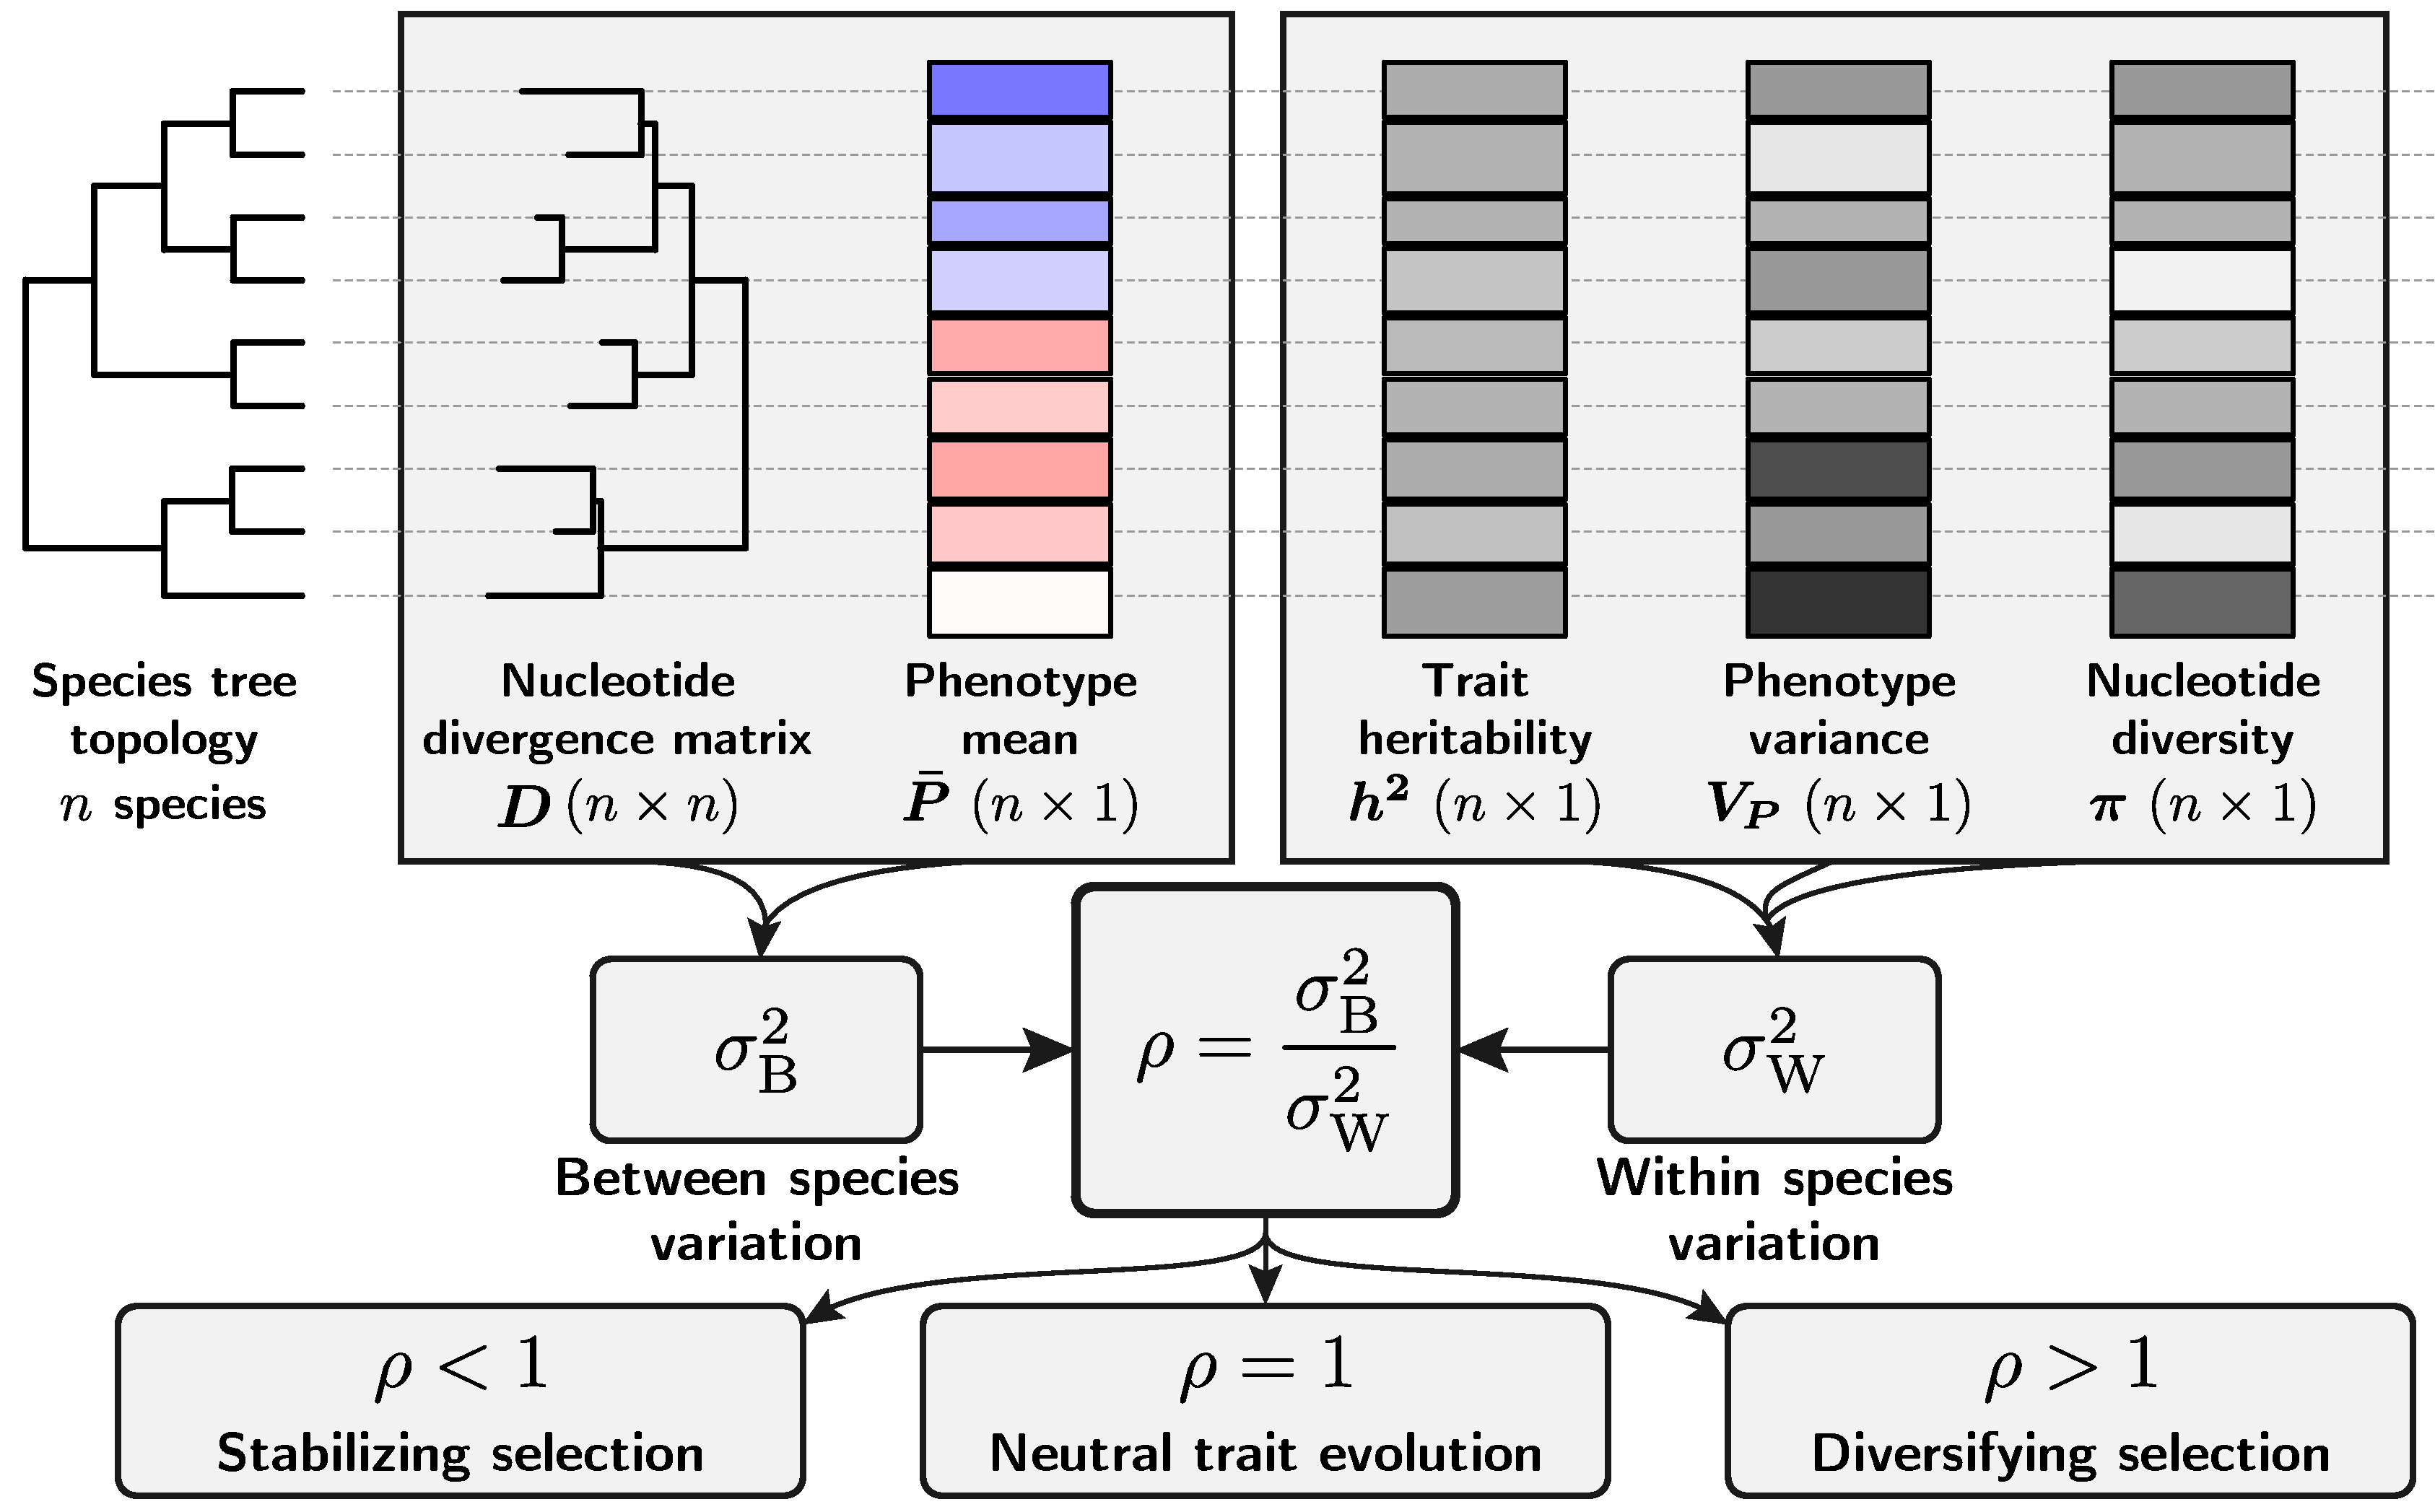
\includegraphics[width=\textwidth, page=1] {figure1}
    \caption{
        Between species, the change along the phylogeny of the mean phenotypic trait allows the estimation of between-species trait variation, \DIFdelbeginFL \DIFdelFL{$\EstRateBetween$}\DIFdelendFL \DIFaddbeginFL \DIFaddFL{$\RateBetween$}\DIFaddendFL , which is normalized by nucleotide divergence.
        Within species, the genetic variance allows the estimation of within-species trait variation, \DIFdelbeginFL \DIFdelFL{$\EstRateWhithin$}\DIFdelendFL \DIFaddbeginFL \DIFaddFL{$\RateWhithin$}\DIFaddendFL , which is  normalized by nucleotide diversity.
        \DIFdelbeginFL \DIFdelFL{$\EstNI$ }\DIFdelendFL \DIFaddbeginFL \DIFaddFL{$\NI$ }\DIFaddendFL is the ratio of \DIFdelbeginFL \DIFdelFL{$\EstRateBetween$ }\DIFdelendFL \DIFaddbeginFL \DIFaddFL{$\RateBetween$ }\DIFaddendFL over \DIFdelbeginFL \DIFdelFL{$\EstRateWhithin$}\DIFdelendFL \DIFaddbeginFL \DIFaddFL{$\RateWhithin$}\DIFaddendFL .
        Under neutral evolution, \DIFdelbeginFL \DIFdelFL{$\EstNI$ }\DIFdelendFL \DIFaddbeginFL \DIFaddFL{$\NI$ }\DIFaddendFL is expected to be equal to one.
        Under diversifying selection, the trait is heterogeneous between species, but homogeneous within species, leading to \DIFdelbeginFL \DIFdelFL{$\EstNI$ }\DIFdelendFL \DIFaddbeginFL \DIFaddFL{$\NI$ }\DIFaddendFL greater than one.
        Under stabilizing selection, the trait is homogeneous between species, leading to \DIFdelbeginFL \DIFdelFL{$\EstNI$ }\DIFdelendFL \DIFaddbeginFL \DIFaddFL{$\NI$ }\DIFaddendFL smaller than one.
        Importantly, the sequence from which nucleotide diversity and divergence are estimated should be neutrally evolving, but they are not necessarily linked to the quantitative trait under study, they allow for discarding the confounding effect on mutation rate diversity, population size and divergence time.
    }
    \label{fig:methods}
\end{figure*}

\subsubsection*{Neutrality index}

The variability between either individuals or species can be obtained for both quantitative traits and genomic sequences.
At the population level, the variability of the trait between individuals can be combined with the nucleotide diversity of any neutrally evolving genomic region to obtain $\RateWhithin$.
At the phylogenetic level, the variability of the mean trait value between species can be combined with the nucleotide divergence of any neutrally evolving genomic region to obtain $\RateBetween$.
If the trait is neutrally evolving and the genetic architecture of the trait has not changed along the phylogenetic tree, we thus have:
\begin{align}
    \frac{\RateBetween}{\RateWhithin} &= \frac{\VarPhy}{4 \NucDiv} \Multiply \frac{\pi}{\Heritability \Multiply \VarPhenotype} \text{ by definition and eq.~\ref{eq:def-rate-pheno-pop} and~\ref{eq:def-rate-phy}},\\
    &= \frac{\MutationRatePheno \Multiply \GenArchi}{\MutationRateNuc} \Multiply \frac{\MutationRateNuc}{\MutationRatePheno \Multiply \GenArchi} \text{ from eq.~\ref{eq:rate-pheno-pop} and~\ref{eq:rate-phy}}, \\
    &= 1.
\end{align}
We define a neutrality index $\NI$ as:
\begin{align}
\NI \defEqual \frac{\RateBetween}{\RateWhithin},
\end{align}
 which will equal to $1$ for a trait evolving neutrally.
Both $\RateBetween$ and $\RateWhithin$ can be estimated using quantitative trait and genomic sequences within and between species, while neither the mutation rates ($\MutationRatePheno$ and $\MutationRateNuc$), nor the effective population size ($\Ne$), generation time or time of divergence ($\NbrGen$) need to be estimated.
Moreover, the nucleotide sequence from which $\pi$ and $\NucDiv$ are obtained should be neutrally evolving, but they are not necessarily linked to the quantitative trait under study.

\subsection*{Estimation}\label{subsec:estimate}

We \DIFdelbegin \DIFdel{denote $\EstNI$, $\EstRateBetween$ and $\EstRateWhithin$ the }\DIFdelend \DIFaddbegin \DIFadd{hereby seek to obtain }\DIFaddend point estimates of \DIFdelbegin \DIFdel{respectively $\NI$, }\DIFdelend $\RateBetween$\DIFdelbegin \DIFdel{and }\DIFdelend \DIFaddbegin \DIFadd{, }\DIFaddend $\RateWhithin$ \DIFaddbegin \DIFadd{and ultimately $\NI$}\DIFaddend .
For each species with data available, $\RateWhithin$ as defined in eq.~\ref{eq:def-rate-pheno-pop} can be seen as a replicate sample.
Thus, \DIFdelbegin \DIFdel{$\EstRateWhithin$ }\DIFdelend \DIFaddbegin \DIFadd{$\RateWhithin$ }\DIFaddend can be obtained by averaging out across all the sampled species.
On the other hand, $\RateBetween$ such as as defined in eq.~\ref{eq:def-rate-phy} only refers to a pair of species, and thus must be generalized to account for different species divergence, as is done in the comparative framework~\citep{felsenstein_phylogenies_1985, omeara_testing_2006}.
Generally, \DIFdelbegin \DIFdel{$\EstRateWhithin$ }\DIFdelend \DIFaddbegin \DIFadd{$\RateBetween$ }\DIFaddend can thus be seen as an estimate of the rate of evolution of the quantitative trait along a phylogenetic tree, when the tree is measured in units of $4d$ ($d$ being the nucleotide divergence).
As such, any phylogenetic comparative methods that allow the estimation of phenotypic rates of evolution on a tree scaled by $4d$, instead of time as is usually the case, can be used to estimate \DIFdelbegin \DIFdel{$\EstRateWhithin$}\DIFdelend \DIFaddbegin \DIFadd{$\RateWhithin$}\DIFaddend .
We provide a maximum likelihood estimate for $\NI$ as well as a Bayesian estimate to derive posterior probabilities that the null model of neutrality (i.e.~$\NI = 1$) is rejected.

\subsubsection*{Maximum likelihood estimate}
At the phylogenetic scale, for $\NbrTaxa$ taxa in the tree, $\DistanceMatrix$ ($\NbrTaxa \times \NbrTaxa$) is the symmetric distance matrix computed from the branch lengths and the topology of the phylogenetic tree.
The diagonal $\Distance_{\Spi,\Spi}$ represents the total nucleotide divergence from the root of the tree to each taxon ($\Spi$).
The off-diagonal elements ($\Distance_{\Spi,\Spj} = \NucDiv$) are the distances between the root and the most recent common ancestor of taxa $\Spi$ and $\Spj$, as in equation~\ref{eq:distance}.
The mean trait value at the root of the tree ($\RootTrait$) can be estimated from the $\NbrTaxa \times 1$ vector of mean trait values $\VecTrait$ at the tips of the tree using maximum likelihood~\citep{omeara_testing_2006}:
\begin{gather}
    \RootTrait = \left( \VecOne\tr \MultiplyMatrix \DistanceMatrix\inv \MultiplyMatrix \VecOne \right)\inv \Multiply \left( \VecOne\tr \MultiplyMatrix \DistanceMatrix\inv \MultiplyMatrix \VecTrait \right), \label{eq:estimated-root-trait}
\end{gather}
where $\VecOne$ is an $\NbrTaxa \times 1$ column vector of ones.

Finally, between-species variation \DIFdelbegin \DIFdel{$\EstRateBetween$ }\DIFdelend \DIFaddbegin \DIFadd{$\RateBetween$ }\DIFaddend is estimated as~\citep{omeara_testing_2006}:
\begin{gather}
    \DIFdelbegin %DIFDELCMD < \EstRateBetween %%%
\DIFdelend \DIFaddbegin \DIFadd{\RateBetween }\DIFaddend = \frac{1}{4}\frac{\left( \VecTrait -  \RootTrait \Multiply \VecOne \right)\tr \MultiplyMatrix \DistanceMatrix\inv \MultiplyMatrix \left( \VecTrait -  \RootTrait \Multiply \VecOne  \right)}{\NbrTaxa - 1}. \label{eq:estimated-rate-phy}
\end{gather}

For a given species $\Spi$ with inter-individual data available, additive genetic variance of a trait ($\VarGeneticSpi$) is the product of heritability ($\Heritability_{i}$) and phenotypic variance ($V_{\Trait, i}$).
The ratio of $\VarGeneticSpi$ over nucleotide diversity of neutrally evolving sequences ($\pi_{\Spi}$) is a sample estimate of $\RateWhithin$.
Averaged across all species, we obtain the estimate \DIFdelbegin \DIFdel{$\EstRateWhithin$ as:
}\DIFdelend \DIFaddbegin \DIFadd{$\RateWhithin$ as:
}\DIFaddend \begin{gather}
    \DIFdelbegin %DIFDELCMD < \EstRateWhithin %%%
\DIFdelend \DIFaddbegin \DIFadd{\RateWhithin }\DIFaddend = \dfrac{1}{\NbrTaxa}\sum_{i=1}^{\NbrTaxa}\frac{  \VarGeneticSpi}{ \pi_{i}} = \dfrac{1}{\NbrTaxa}\sum_{i=1}^{\NbrTaxa} \frac{  V_{\Trait, i} \Multiply \Heritability_{i}}{ \pi_{i}}. \label{eq:estimated-rate-pop}
\end{gather}

As depicted in fig.~\ref{fig:methods}, the neutrality index is estimated as:
\begin{gather}
    \DIFdelbegin %DIFDELCMD < \EstNI %%%
\DIFdelend \DIFaddbegin \DIFadd{\NI }\DIFaddend = \DIFdelbegin \DIFdel{\frac{\EstRateBetween}{\EstRateWhithin}}\DIFdelend \DIFaddbegin \DIFadd{\frac{\RateBetween}{\RateWhithin}}\DIFaddend . \label{eq:estimated-NI}
\end{gather}

\subsubsection*{Multivariate Brownian process}

In the previous section, \DIFdelbegin \DIFdel{$\EstNI$ }\DIFdelend \DIFaddbegin \DIFadd{$\NI$ }\DIFaddend is estimated independently for each trait of interest.
Here we generalize to $\Ntrait$ traits co-varying along the phylogenetic tree\DIFdelbegin \DIFdel{.
Trait }\DIFdelend \DIFaddbegin \DIFadd{, since simultaneously estimating all $\RateBetween$ allows improving their estimation~\mbox{%DIFAUXCMD
\citep{adams_multivariate_2018}}\hskip0pt%DIFAUXCMD
.
More specifically, trait }\DIFaddend variation along the phylogenetic tree is modeled as a $\Ntrait$-dimensional Brownian process $\Brownian$ ($1 \times \Ntrait$) starting at the root and branching along the tree topology~\citep{huelsenbeck_detecting_2003, lartillot_phylogenetic_2011, lartillot_joint_2012, latrille_inferring_2021}.
The rate of change of the Brownian process is determined by the positive semi-definite and symmetric covariance matrix between traits $\CovarianceMatrix$ ($\Ntrait \times \Ntrait$).
The branch lengths of the tree used to model the Brownian process runs is measured in units of $4d$ ($d$ being the nucleotide divergence).
The off-diagonal elements of $\CovarianceMatrix$ are the covariance between traits, and the diagonal elements are the variance of each trait when measured in $4d$ units, and thus equate to \DIFdelbegin \DIFdel{$\EstRateBetween$ }\DIFdelend \DIFaddbegin \DIFadd{$\RateBetween$ }\DIFaddend (see section~S\ref{subsec:multivariate-brownian-process}).
\DIFaddbegin \DIFadd{Of note, modeling trait evolution as a multi-dimensional process is reliable only if $\Ntrait \ll \NbrTaxa$, meaning that the number of species is largely superior to the number of traits~\mbox{%DIFAUXCMD
\citep{adams_multivariate_2018}}\hskip0pt%DIFAUXCMD
.
Thus, relying on a $\Ntrait$-dimensional process should be reserved for a handful of allometric traits (e.g. brain mass and body mass).
If $\Ntrait$ is large, the traits are better tested independently each with a $1$-dimensional Brownian process, which is a specific case of the multi-dimensional process.
}\DIFaddend 

\subsubsection*{Bayesian estimate}
The Bayesian framework allows obtaining the posterior distribution of neutrality index (\DIFdelbegin \DIFdel{$\EstNI$}\DIFdelend \DIFaddbegin \DIFadd{$\NI$}\DIFaddend ) for traits of interest.
We used the \textit{BayesCode} software to model $\Ntrait$-dimensional Brownian processes along a phylogenetic tree~\citep{latrille_inferring_2021}.
With an inverse Wishart distribution as the {prior} on the covariance matrix, the {posterior} on $\CovarianceMatrix$, conditional on $\brownian$ is also an invert Wishart distribution (see section~S\ref{subsec:sampling-the-covariance-matrix}).
We used Metropolis-Hastings algorithm to sample $\Brownian$, while the posterior distribution of $\CovarianceMatrix$ is sampled using Gibbs sampling.
For each trait and each species, the prior on heritability ($\Heritability$) for each species is set as a uniform distribution with user-defined boundaries.
Heritability and phenotypic variance for each trait are combined with nucleotide diversity to compute \DIFdelbegin \DIFdel{$\EstRateWhithin$ }\DIFdelend \DIFaddbegin \DIFadd{$\RateWhithin$ }\DIFaddend for each species before being averaged across species (as in eq.~\ref{eq:estimated-rate-pop}).
From \DIFdelbegin \DIFdel{$\EstRateWhithin$ and }\DIFdelend \DIFaddbegin \DIFadd{$\RateWhithin$ estimated independently for each trait and the diagonal elements of }\DIFaddend $\CovarianceMatrix$ \DIFaddbegin \DIFadd{(i.e. the $\RateBetween$ for each trait)}\DIFaddend , the posterior distribution of \DIFdelbegin \DIFdel{$\EstNI$ }\DIFdelend \DIFaddbegin \DIFadd{$\NI$ }\DIFaddend (as in eq.~\ref{eq:estimated-NI}) is obtained for each trait.
The posterior distribution of \DIFdelbegin \DIFdel{$\EstNI$ }\DIFdelend \DIFaddbegin \DIFadd{$\NI$ }\DIFaddend thus allows testing for deviation from neutrality (Fig.~\ref{fig:methods}), for example, by computing \DIFdelbegin \DIFdel{$\proba [\EstNI > 1 ]$ }\DIFdelend \DIFaddbegin \DIFadd{$\proba [\NI > 1 ]$ }\DIFaddend to test for evidence of diversifying selection and \DIFdelbegin \DIFdel{$\proba [\EstNI < 1 ]$ }\DIFdelend \DIFaddbegin \DIFadd{$\proba [\NI < 1 ]$ }\DIFaddend to test for evidence of stabilizing selection.

\subsubsection*{Applicability to empirical data}

Our method assumes that the narrow-sense heritability ($\Heritability$) of a trait is known such as to estimate additive genetic variance ($\VarGenetic$) from phenotypic variance ($\VarPhenotype$) as $\VarGenetic = \Heritability \Multiply \VarPhenotype$.
Fortunately, if heritability is not known, the test for diversifying selection can still be performed, although it is underpowered.
Indeed, if the additive genetic variance is substituted by phenotypic variance, it is equivalent to assuming complete heritability ($\Heritability = 1$).
Because $\Heritability \leq 1$ by definition, we overestimate the within-species variation and thus underestimate \DIFdelbegin \DIFdel{$\EstNI$}\DIFdelend \DIFaddbegin \DIFadd{$\NI$}\DIFaddend .
It is, however, possible to test for diversifying selection because testing for \DIFdelbegin \DIFdel{$\EstNI > 1$ }\DIFdelend \DIFaddbegin \DIFadd{$\NI > 1$ }\DIFaddend while using phenotypic variance instead of additive genetic variance means that knowing the additive genetic variance would have only increased the evidence for diversifying selection.
\DIFaddbegin \DIFadd{Similarly, using the broad-sense heritability ($H^2$) instead of narrow-sense heritability ($\Heritability$) results in an underestimation of $\NI$ since $\Heritability \leq H^2$ and thus can be used to detect diversifying selection if $\Heritability$ is not available.
}\DIFaddend Additionally, empirical estimates of $\Heritability$ are surprisingly stable across species and fall within the range of 0.2-0.5 in a vast majority of phenotypic traits tested~\citep{hansen_heritability_2011, hansen_evolvability_2021}.
\DIFdelbegin \DIFdel{Alternatively, using the broad-sense heritability ($H^2$) instead of narrow-sense heritability ($\Heritability$) results in an underestimation of $\EstNI$ since $\Heritability \leq H^2$.
If }\DIFdelend \DIFaddbegin \DIFadd{Thus, if }\DIFaddend available, such prior knowledge on $\Heritability$ can be leveraged instead of assuming complete heritability to increase the statistical power to detect diversifying selection.

In contrast to the test of diversifying selection, the test for stabilizing selection is invalid if \DIFdelbegin \DIFdel{$\EstNI$ }\DIFdelend \DIFaddbegin \DIFadd{$\NI$ }\DIFaddend is underestimated.
Several assumptions made by our test might not hold on empirical data and their consequences on the neutrality index and the test that can be performed are shown in Table~\ref{table:assumptions}.

\subsection*{Simulation}\label{subsec:simulations}

% vG: 13.8, vP: 69.0, vE: 55.2, nbr_loci: 5000, a: 1.0, mut_rate: 1.38e-05, pop_size: 50, h2: 0.2
% pS = 0.0027577478571428568
% Tree length (dS) = 2.340579
% Tree length (My) = 1259.4490200000002
% Root age (My) = 98.9489413888889
% Root age (dS) = 0.18388820079995308
% nbr_sites_var = 27.577478571428568
% u = 1.3788739285714283e-05
% nbr_generations = 13336.114128321291
We tested the performance of our neutrality index ($\NI$) to detect selection on a quantitative trait using simulations.
We performed simulations under different selective regimes (neutral, stabilizing, diversifying), different demographic histories (constant or fluctuating population size) and different evolution of the mutation rate (constant or fluctuating).
Simulations were individual-based and followed a Wright-Fisher model with mutation, selection and drift for a diploid population including speciation along a predefined ultrametric phylogenetic tree (Fig.~\ref{fig:simulator}A\&B).
Each individual phenotypic value was the sum of genotypic value and an environmental effect.
The environmental effect was normally distributed with variance $\VarEnv$.
We assumed that the genotypic value was encoded by $\NbrLoci=5,000$ loci, with each locus contributing an additive effect that was normally distributed with standard deviation $a=1$ (Fig.~\ref{fig:simulator}A and for the theoretical formulation see section~S\ref{subsec:genotype-phenotype-map} and fig.~\ref{fig:simulator-summary}).
We assumed a trait with a narrow-sense heritability of $\Heritability=0.2$ and computed the theoretical $\VarEnv$ accordingly (see section~S\ref{subsec:genotype-phenotype-map}).
Assuming a diploid panmictic population of size $\Ne=50$ at the root of the tree, and with non-overlapping generations, we simulated explicitly each generation along an ultrametric phylogenetic tree.
For each offspring, the number of mutations was drawn from a Poisson distribution with mean $2 \Multiply \MutationRatePheno \Multiply \NbrLoci $, with the mutation rate per locus per generation $\MutationRatePheno$.
From the empirical mammalian dataset (see next section), we computed an average nucleotide divergence from the root to leaves of $0.18$ and average genetic diversity of $0.00276$.
We scaled parameters in our simulations to fit plausible values for mammals.
We thus used a nucleotide mutation rate of $\MutationRateNuc=0.00276 / 4 \Ne = 1.38 \times 10^{-5}$ per site per generation  and a total of $0.18 / 1.38 \times 10^{-5} = 13,500$ generations from root to leaves, and the number of generations along each branch was proportional to the branch length.
We set $\MutationRatePheno=\MutationRateNuc$ without loss in generality since the genetic architecture ($\NbrLoci$ and $a$) is assumed constant in the simulator.

The changes in $\MutationRatePheno$ and $\Ne$ along the lineages were both modeled by a Brownian process on the log scale (log-$\MutationRatePheno$ and log-$\Ne$), leading to geometric Brownian motion on the linear scale ($\MutationRatePheno$ and $\Ne$).
These processes are parameterized as $\brownian \left(0, \sigma_{\MutationRatePheno}=0.0086\right)$ and $\brownian \left(0, \sigma_{\Ne}=0.0086\right)$, which, if counted across $13,500$ generations, leads to a standard deviation of $0.0086 \Multiply \sqrt {13,500} = 1.0$.
In other words, the deviation in log-$\Ne$ and log-$\MutationRatePheno$  between the extant species and the root is $1.0$.
An Ornstein-Uhlenbeck process was overlaid to the instant value of log-$\Ne$ provided by the geometric Brownian process to account for short-term changes between generations ($\text{OU} \left(0, \sigma_{\Ne}=0.1, \theta_{\Ne}=0.9\right)$).
The geometric Brownian motion accounted for long-term fluctuations (low rate of changes $\sigma_{\Ne}$ but unbounded), while the Ornstein-Uhlenbeck introduced short-term fluctuations (high rate of changes $\sigma_{\Ne}$ but bounded and mean-reverting).
The simulation started from an initial sequence at equilibrium at the root of the tree and, at each node, the process was split until it finally reached the leaves of the tree.
From a speciation process perspective, this was equivalent to an allopatric speciation over one generation.

At each generation, parents were randomly sampled with a weight proportional to their fitness ($W$).
Selection was modeled as a one-dimensional Fisher's geometric landscape, with the fitness of an individual being a monotonously decreasing function of the distance between the individual and the optimal phenotype~\citep{tenaillon_utility_2014,blanquart_epistasis_2016}.
More specifically, the fitness of an individual was given by $W = \e^{(\Trait - \lambda)^2/ \alpha}$, where $\Trait$ was the trait value of the individual, $\lambda=0.0$ was the optimal trait value, and $\alpha=0.02$ was the strength of selection.
Mutations were considered as a displacement of the phenotype in the multidimensional space.
Beneficial mutations moved the phenotype closer to the optimum, while deleterious mutations moved it further away.
Stabilizing selection was implemented by fixing the optimum phenotype to a single value ($\lambda=0.0$).
Diversifying selection was implemented by allowing the optimum phenotype to move along the phylogenetic tree as a geometric Brownian process~\citep{hansen_stabilizing_1997} ($\lambda \sim \brownian \left(0, \sigma_{\lambda}=1.0\right)$).
Neutral evolution was implemented by \DIFdelbegin \DIFdel{fixing }\DIFdelend \DIFaddbegin \DIFadd{flattening }\DIFaddend the fitness landscape ($W=1$), which meant that each individual had the same probability of being sampled at each generation.

Nucleotide diversity ($\pi$) was measured as the heterozygosity of neutral markers that were simulated along the phylogenetic tree but not linked to the trait simulated.
Nucleotide divergence ($d$) was measured as the number of substitutions per site of neutral markers along the branches of the phylogenetic tree.
The additive genetic variance was measured as phenotypic variance multiplied by heritability.
Heritability was estimated from the slopes of the regression of offspring's phenotypic trait values on parental phenotypic trait values~\citep{lynch_genetics_1998} averaged over the last 10 simulated generations.
Heritability was thus not a given parameter of the simulations, but rather measured as it would be in empirical data.

\begin{figure*}[!ht]
    \centering
    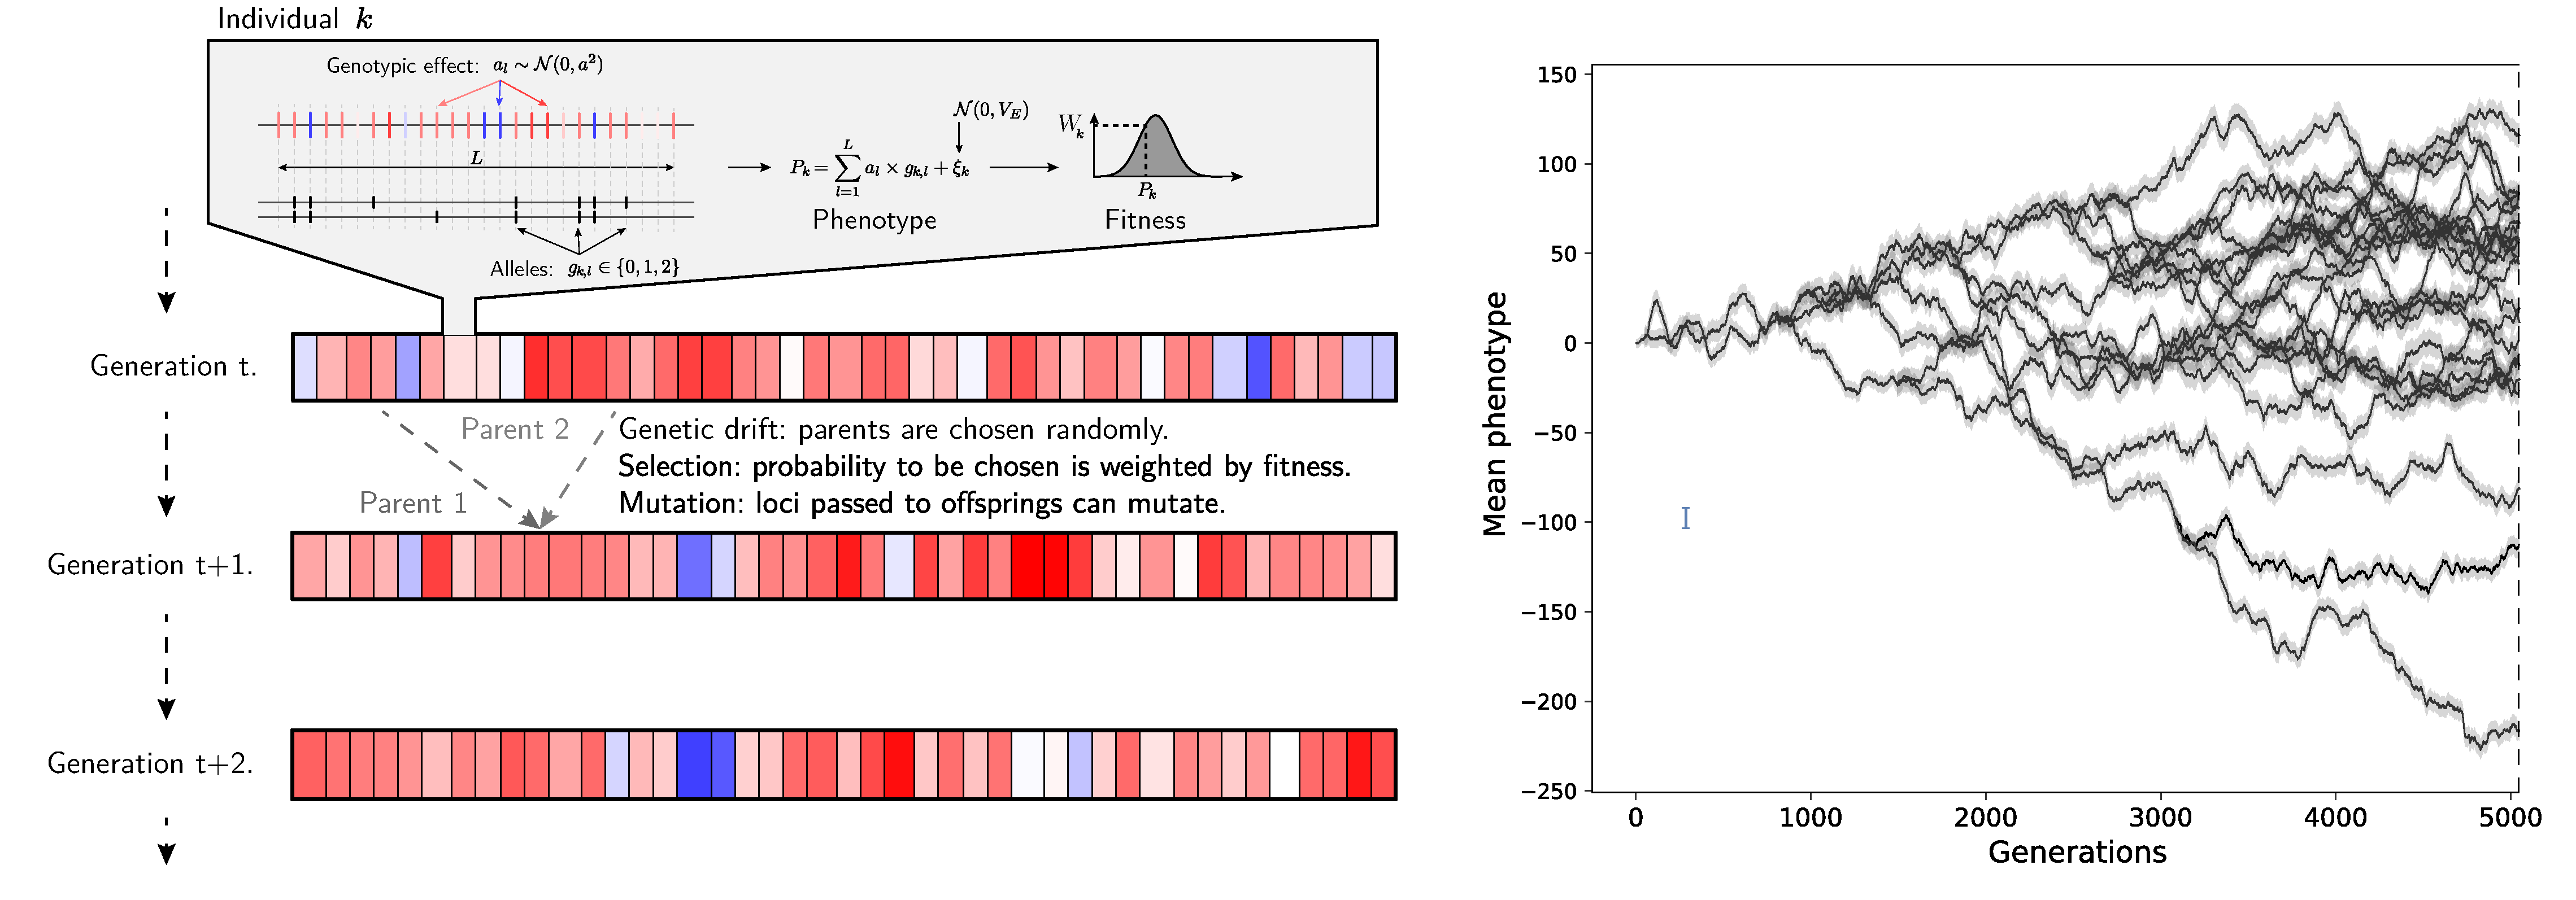
\includegraphics[width=\textwidth, page=1] {figure2}
    \caption{
        Wright-Fisher simulations with mutation, selection and drift.
        Left panel: For a given individual, the trait phenotypic value is the sum of genotypic value and a environmental effect (standard deviation $\VarEnv$).
        The trait's genotypic value is encoded by $\NbrLoci$ independent loci (meaning no linkage), with each locus contributing additively to the genotypic value.
        Parents are selected for reproduction to the next generation according to their phenotypic value, with a probability proportional to their fitness.
        Mutations are drawn from a Poisson distribution, with each locus having a probability $\MutationRatePheno$ to mutate.
        Drift is modeled by the resampling of parents.
        Right panel: examples of a trait evolving along a phylogenetic tree, with the mean phenotype (black line) and the variance of the trait genotypic value (gray area).
    }
    \label{fig:simulator}
\end{figure*}

\subsection*{Empirical dataset}\label{subsec:empirical-dataset}

We analyzed a dataset of body and brain masses from mammals.
The log-transformed values of body and brain masses were taken from \citet{tsuboi_breakdown_2018}.
We removed individuals not marked as adults and split the data into males and females due to sexual dimorphism in body and brain masses.
We discarded species with only one representative since phenotypic variance cannot be estimated.
The mammalian genomic data are gathered from the Zoonomia project~\citep{genereux_comparative_2020}.
More specifically, nucleotide divergence is estimated on a set of neutral markers in \citet{foley_genomic_2023}, and with nucleotide diversity measured as heterozygosity in \citet{wilder_contribution_2023}.

We also analyzed a dataset of primate species, with the nucleotide variation obtained from \citet{kuderna_global_2023} and the quantitative trait variation also from \citet{tsuboi_breakdown_2018}, using the same filtering as for the mammalian dataset.
However, the primate nucleotide divergence was not obtained on a set of neutral markers as for the mammalian dataset, but across the whole genome.
As such, the evidence for \DIFdelbegin \DIFdel{$\EstNI > 1$ }\DIFdelend \DIFaddbegin \DIFadd{$\NI > 1$ }\DIFaddend does not necessarily imply that the trait is evolving under diversifying selection since non-neutral markers included in the estimate of divergence can lead to a spurious \DIFdelbegin \DIFdel{$\EstNI > 1$ }\DIFdelend \DIFaddbegin \DIFadd{$\NI > 1$ }\DIFaddend (see table~\ref{table:assumptions}).

\section*{Results}\label{sec:results}

\subsection*{Neutrality index}

For a neutral trait, the genetic architecture, meaning the number of loci encoding the trait and the average effect of a mutation on the trait, is formally related to both within and between-species variation of the trait.
We defined the neutrality index as $\NI = \RateBetween/\RateWhithin$, which equals $1$ for a neutral trait (see Materials and Methods), suggesting that traits for which this relationship was not verified were putatively under selection.
Under stabilizing selection, the variation between species is depleted because the mean trait is maintained toward similar values between different species, which leads to $\NI < 1$.
In contrast, under diversifying selection, the variation between species is inflated because species will have potentially different trait values~\citep{hansen_stabilizing_1997}, which leads to $\NI > 1$.
Our neutrality index for a quantitative trait leveraged the data for any number of species, and took advantage of the signal over the whole phylogenetic tree, while at the same time taking into account phylogenetic inertia and addressing the non-independence between species (Fig.~\ref{fig:methods}).
This statistic was obtained as a maximum likelihood estimate \DIFdelbegin \DIFdel{($\EstNI$), }\DIFdelend from eq.~\ref{eq:estimated-rate-pop} and~\ref{eq:estimated-rate-phy}.
We also devised a Bayesian estimate to obtain the posterior distribution of the neutrality index, and test for diversifying selection as \DIFdelbegin \DIFdel{$\proba [\EstNI > 1]$}\DIFdelend \DIFaddbegin \DIFadd{$\proba [\NI > 1]$}\DIFaddend , and stabilizing selection as \DIFdelbegin \DIFdel{$\proba [\EstNI < 1]$}\DIFdelend \DIFaddbegin \DIFadd{$\proba [\NI < 1]$}\DIFaddend .

Our neutrality index made a series of assumptions that we described in details in the Material and Methods section.
Table~\ref{table:assumptions} summarized these assumptions and outlined possible consequences for the neutrality test that we proposed.

\subsection*{Results against simulations}\label{subsec:results-against-simulations}

The inference framework was first tested on independently simulated datasets matching an empirically relevant mammalian empirical regime (see Materials and Methods).
Under constant population size ($\Ne$) and constant mutation rates ($\MutationRatePheno$ and $\MutationRateNuc$) across the phylogenetic tree (fig.~\ref{fig:results-simulations}, top row), we found no false negative for simulations of stabilizing (\DIFdelbegin \DIFdel{$\proba [\EstNI < 1] > 0.975$}\DIFdelend \DIFaddbegin \DIFadd{$\proba [\NI < 1] > 0.975$}\DIFaddend ; blue in fig.~\ref{fig:results-simulations}) or diversifying (\DIFdelbegin \DIFdel{$\proba [\EstNI > 1] > 0.975$}\DIFdelend \DIFaddbegin \DIFadd{$\proba [\NI > 1] > 0.975$}\DIFaddend ; red in fig.~\ref{fig:results-simulations}) selection.
For simulations under neutral evolution, 77\% of those were correctly identified (\DIFdelbegin \DIFdel{$0.025 \leq \proba [\EstNI > 1] \leq 0.975$}\DIFdelend \DIFaddbegin \DIFadd{$0.025 \leq \proba [\NI > 1] \leq 0.975$}\DIFaddend ; yellow in fig.~\ref{fig:results-simulations}), while 21\% and 2\% were wrongly detected as stabilizing or diversifying selection, respectively.
Once we introduced fluctuating $\Ne$, $\MutationRatePheno$ and $\MutationRateNuc$(Fig.~\ref{fig:results-simulations}, bottom row), our ability to identify simulations under either diversifying or stabilizing selection remained the same with all cases detected correctly.
For simulations under neutral evolution, 51\% of the simulations were correctly detected (\DIFdelbegin \DIFdel{$0.025 \leq \proba [\EstNI > 1] \leq 0.975$}\DIFdelend \DIFaddbegin \DIFadd{$0.025 \leq \proba [\NI > 1] \leq 0.975$}\DIFaddend ), while 49\% were detected as stabilizing selection (\DIFdelbegin \DIFdel{$\proba [\EstNI < 1] > 0.975$}\DIFdelend \DIFaddbegin \DIFadd{$\proba [\NI < 1] > 0.975$}\DIFaddend ) and none as diversifying selection.

\begin{figure*}[!ht]
    \centering
    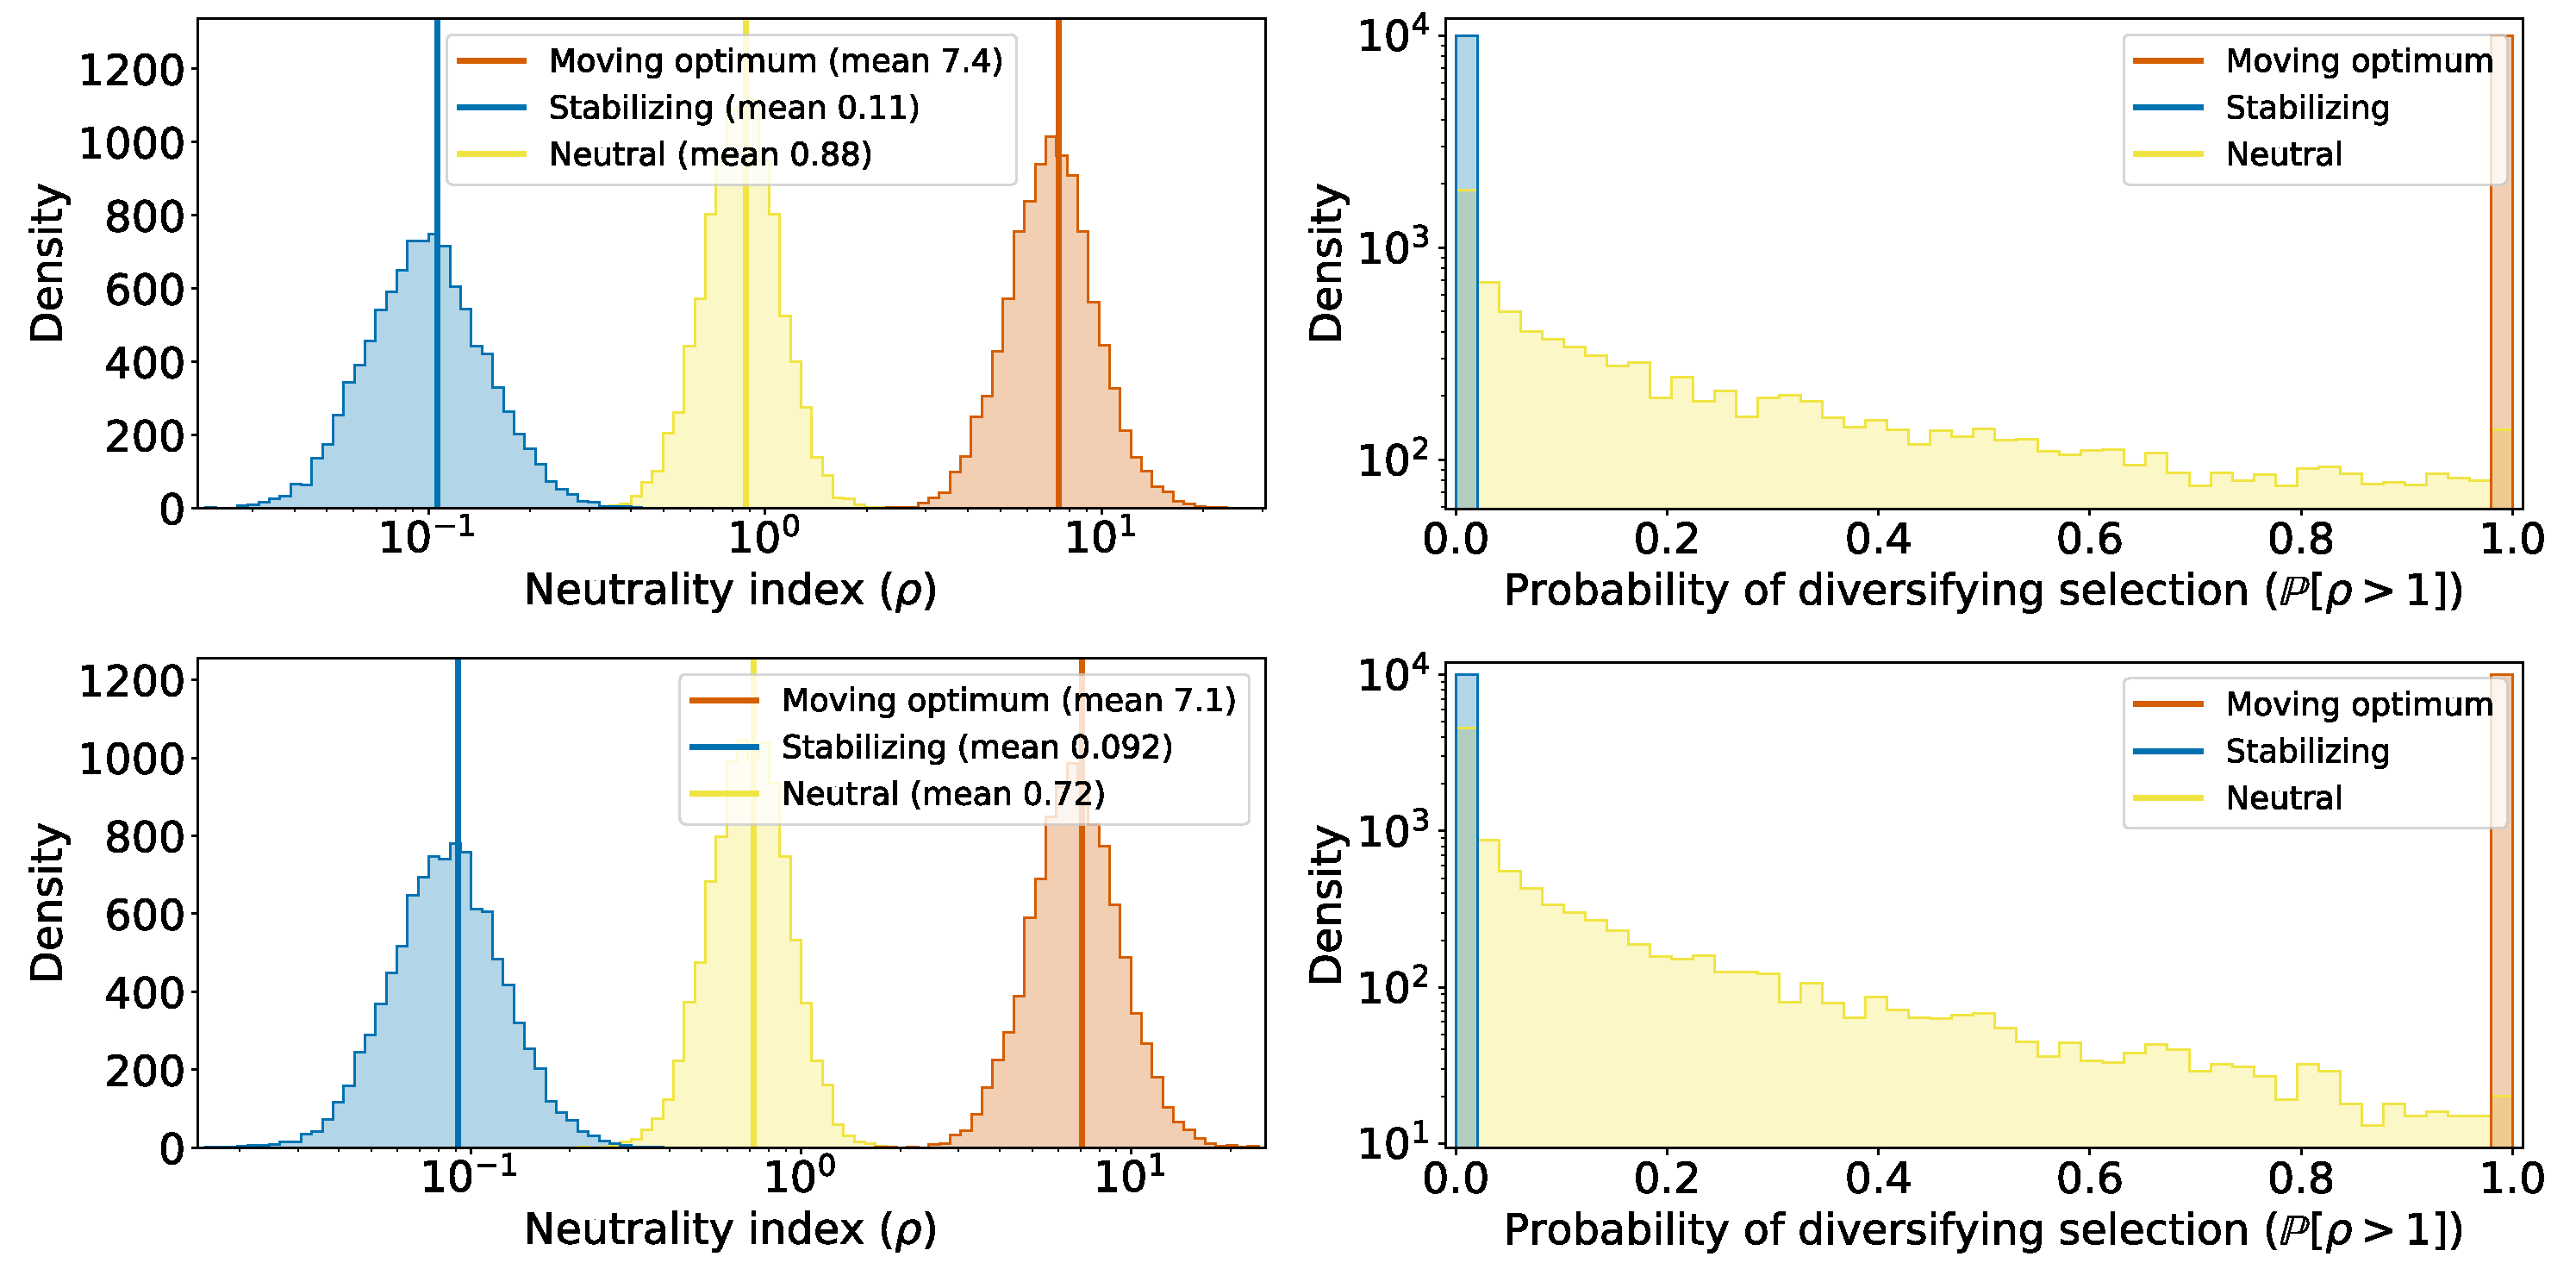
\includegraphics[width=\textwidth, page=1] {figure3}
    \caption{
        $10,000$ simulations of trait evolution along a phylogenetic tree under different selection regimes.
        Traits simulated under stabilizing selection (blue), under a neutral evolution (yellow), and under a moving optimum (red).
        Histogram of ratio of between-species trait variation (\DIFdelbeginFL \DIFdelFL{$\EstRateBetween$}\DIFdelendFL \DIFaddbeginFL \DIFaddFL{$\RateBetween$}\DIFaddendFL ) over within-species trait variation \DIFdelbeginFL \DIFdelFL{$\EstRateWhithin$ }\DIFdelendFL \DIFaddbeginFL \DIFaddFL{$\RateWhithin$ }\DIFaddendFL with \DIFdelbeginFL \DIFdelFL{$\EstNI = \EstRateBetween / \EstRateWhithin$ }\DIFdelendFL \DIFaddbeginFL \DIFaddFL{$\NI = \RateBetween / \RateWhithin$ }\DIFaddendFL estimated from each simulated data (left) and probabilities of \DIFdelbeginFL \DIFdelFL{$\EstNI$ }\DIFdelendFL \DIFaddbeginFL \DIFaddFL{$\NI$ }\DIFaddendFL being greater than $1$ (right).
        Effective population size ($\Ne$) and mutation rates ($\MutationRatePheno$ and $\MutationRateNuc$) were either constant (top row), or fluctuating as a Brownian process along the phylogenetic tree (bottom row).
    }
    \label{fig:results-simulations}
\end{figure*}


\begin{table*}[t!]
    \centering
    \begin{adjustbox}{width = 0.75\textwidth}
        \begin{tabular}{||l|l|l|c|c|c|c|c||}
        \toprule
        Dataset & Trait & $\Heritability$ & Sex & $\NbrTaxa$ & \DIFdelbeginFL \DIFdelFL{$\EstNI$ }\DIFdelendFL \DIFaddbeginFL \DIFaddFL{$\NI$ }\DIFaddendFL & $95\%$ CI for \DIFdelbeginFL \DIFdelFL{$\EstNI$ }\DIFdelendFL \DIFaddbeginFL \DIFaddFL{$\NI$ }\DIFaddendFL & \DIFdelbeginFL \DIFdelFL{$\proba [\EstNI > 1 ]$ }\DIFdelendFL \DIFaddbeginFL \DIFaddFL{$\proba [\NI > 1 ]$ }\DIFaddendFL \\ \hline
        \midrule
        Mammals & Body mass & 1.0 & \Male & 36 & 0.340 & 0.217-0.523 & 0.000 \\ \hline
        Mammals & Body mass & 1.0 & \Female & 26 & 0.277 & 0.160-0.490 & 0.000 \\ \hline
        Mammals & Body mass & $\mathcal{U}(0.2, 0.4)$ & \Male & 36 & 1.124 & 0.721-1.754 & 0.635 \\ \hline
        Mammals & Body mass & $\mathcal{U}(0.2, 0.4)$ & \Female & 26 & 0.936 & 0.523-1.715 & 0.324 \\ \hline \hline
        Mammals & Brain mass & 1.0 & \Male & 36 & 1.351 & 0.851-2.173 & 0.877 \\ \hline
        Mammals & Brain mass & 1.0 & \Female & 26 & 1.727 & 0.991-2.938 & 0.972 \\ \hline
        Mammals & Brain mass & $\mathcal{U}(0.2, 0.4)$ & \Male & 36 & 4.527 & 2.831-7.091 & 1.000 \\ \hline
        Mammals & Brain mass & $\mathcal{U}(0.2, 0.4)$ & \Female & 26 & 6.001 & 3.288-10.941 & 1.000 \\ \hline \hline
        Primates & Body mass & 1.0 & \Male & 71 & 0.558 & 0.401-0.784 & 0.000 \\ \hline
        Primates & Body mass & 1.0 & \Female & 65 & 0.389 & 0.278-0.547 & 0.000 \\ \hline
        Primates & Body mass & $\mathcal{U}(0.2, 0.4)$ & \Male & 71 & 1.875 & 1.288-2.695 & 1.000 \\ \hline
        Primates & Body mass & $\mathcal{U}(0.2, 0.4)$ & \Female & 65 & 1.296 & 0.899-1.821 & 0.914 \\ \hline \hline
        Primates & Brain mass & 1.0 & \Male & 71 & 1.929 & 1.395-2.616 & 1.000 \\ \hline
        Primates & Brain mass & 1.0 & \Female & 65 & 1.950 & 1.399-2.790 & 1.000 \\ \hline
        Primates & Brain mass & $\mathcal{U}(0.2, 0.4)$ & \Male & 71 & 6.479 & 4.658-8.944 & 1.000 \\ \hline
        Primates & Brain mass & $\mathcal{U}(0.2, 0.4)$ & \Female & 65 & 6.522 & 4.664-9.294 & 1.000 \\
        \bottomrule
        \end{tabular}
    \end{adjustbox}
    \caption{
    Test of diversifying selection on a mammal and a primate dataset, by splitting males (\Male) and females (\Female).
    Traits considered were body mass or brain mass (log-transformed).
    Heritability ($\Heritability$) was either assumed complete ($\Heritability=1.0$) or uniformly distributed between 20\% and 40\%  ($\Heritability \sim \mathcal{U}(0.2, 0.4)$).
    $\NbrTaxa$ was the number of species in the dataset.
    \DIFdelbeginFL \DIFdelFL{$\EstNI$ }\DIFdelendFL \DIFaddbeginFL \DIFaddFL{$\NI$ }\DIFaddendFL was the posterior estimate of our neutrality index, with the $95\%$ credible interval (CI) for \DIFdelbeginFL \DIFdelFL{$\EstNI$ }\DIFdelendFL \DIFaddbeginFL \DIFaddFL{$\NI$ }\DIFaddendFL also computed.
    \DIFdelbeginFL \DIFdelFL{$\proba [\EstNI > 1 ]$ }\DIFdelendFL \DIFaddbeginFL \DIFaddFL{$\proba [\NI > 1 ]$ }\DIFaddendFL was the estimated posterior probability of diversifying selection.
    }
    \label{table:empirical}
\end{table*}

\subsection*{Results on empirical data}\label{subsec:results-on-empirical-data}

For mammalian body and brain mass, we obtained male (\Male) and female (\Female) trait variations.
Combined with nucleotide diversity and divergence, we estimated \DIFdelbegin \DIFdel{$\EstNI$ }\DIFdelend \DIFaddbegin \DIFadd{$\NI$ }\DIFaddend and posterior probabilities of diversifying selection under different assumptions for trait heritability as shown in the Table~\ref{table:empirical}.
Assuming complete heritability, \DIFdelbegin \DIFdel{brain }\DIFdelend \DIFaddbegin \DIFadd{body }\DIFaddend mass was found to be under diversifying selection with posterior probabilities of $0.0$ for both males and females.
If we assumed that heritability ($\Heritability$) of body mass was uniformly distributed between 20\% and 40\%~\citep{hu_bringing_2022}, posterior probabilities of diversifying selection became $0.635$ for males and $0.324$ for females.
Mammalian brain mass was found to be under diversifying selection with posterior probabilities of $0.877$ for males and $0.972$ for females when complete heritability was assumed.
Assuming a uniform distribution between 20\% and 40\% for heritability led to posterior probabilities of diversifying selection of $1.0$ for both males and females.

We also analyzed a similar dataset for body mass focusing this time only at Primates (Table~\ref{table:empirical}).
For primates body mass, \DIFaddbegin \DIFadd{assuming complete heritability, body mass was found to be under diversifying selection with posterior probabilities of $0.0$ for both males and females, exactly as in the mammal dataset.
However, }\DIFaddend we found posterior probabilities of diversifying selection of $1.0$ for males and $0.914$ for females when assuming a uniform distribution for the heritability of body mass between 20\% and 40\%.
\DIFdelbegin \DIFdel{Assuming complete heritability of body mass }\DIFdelend \DIFaddbegin \DIFadd{For brain mass, assuming complete heritability or not (between 20\% and 40\%) }\DIFaddend did not change the posterior probability \DIFdelbegin \DIFdel{for males, but increased the one for female to }\DIFdelend \DIFaddbegin \DIFadd{of diversifying selection, which was }\DIFaddend $1.0$.
Evidence for diversifying selection on \DIFaddbegin \DIFadd{both brain and }\DIFaddend body mass was therefore more pronounced in Primates than in mammals.
However, the genetic markers used to normalize trait variance with nucleotide divergence were not necessarily neutral, which could create spurious false positives by artificially inflating \DIFdelbegin \DIFdel{$\EstNI$ }\DIFdelend \DIFaddbegin \DIFadd{$\NI$ }\DIFaddend (Table~\ref{table:assumptions} and methods).

\begin{table*}[t!]
    \centering
    \begin{adjustbox}{width = 1.0\textwidth}
        \begin{tabular}{||l|l||c|c||c|c||}
            \hline
            Broken assumption                                       & Consequences                                       & \DIFdelbeginFL \DIFdelFL{$\EstRateWhithin$   }\DIFdelendFL \DIFaddbeginFL \DIFaddFL{$\RateWhithin$   }\DIFaddendFL & \DIFdelbeginFL \DIFdelFL{$\EstRateBetween$   }\DIFdelendFL \DIFaddbeginFL \DIFaddFL{$\RateBetween$   }\DIFaddendFL & Test \DIFdelbeginFL \DIFdelFL{$\EstNI > 1$ }\DIFdelendFL \DIFaddbeginFL \DIFaddFL{$\NI > 1$ }\DIFaddendFL & Test \DIFdelbeginFL \DIFdelFL{$\EstNI < 1$ }\DIFdelendFL \DIFaddbeginFL \DIFaddFL{$\NI < 1$ }\DIFaddendFL \\ \hline \hline
            Trait encoded by few loci                        & Between-species trait variation is underestimated & --              & Underestimated & Conservative & Invalid  \\ \hline
            Sexual dimorphism                                & Within-species trait variation is overestimated   & Overestimated & -- & Conservative & Invalid  \\ \hline
            Phenotypic plasticity & Trait responding to individual environments  & Overestimated & -- & Conservative & Invalid  \\ \hline
            Inbreeding                                       & Nucleotide diversity ($\pi$) is underestimated    & Overestimated  & --              & Conservative & Invalid  \\ \hline
            Markers for polymorphism are negatively selected & Nucleotide diversity ($\pi$) is underestimated  & Overestimated & -- & Conservative & Invalid  \\ \hline
            Markers for polymorphism are positively selected & Nucleotide diversity ($\pi$) is underestimated  & Overestimated & -- & Conservative & Invalid  \\ \hline
            Markers for divergence are positively selected   & Nucleotide divergence ($d$) is overestimated & -- & Underestimated & Conservative & Invalid  \\ \hline
            Markers for polymorphism under balanced selection & Nucleotide diversity ($\pi$) is overestimated  & Underestimated & -- & Invalid & Conservative  \\ \hline
            Markers for divergence are negatively selected   & Nucleotide divergence ($d$) is underestimated & -- & Overestimated & Invalid & Conservative  \\ \hline
            Multiple nucleotide substitutions at the same locus & Nucleotide divergence ($d$) is underestimated & -- & Overestimated & Invalid & Conservative  \\\hline \hline
        \end{tabular}
    \end{adjustbox}
    \caption{Assumptions breaks and their consequences on the estimation of within-species variation (\DIFdelbeginFL \DIFdelFL{$\EstRateWhithin$}\DIFdelendFL \DIFaddbeginFL \DIFaddFL{$\RateWhithin$}\DIFaddendFL ), between-species variation (\DIFdelbeginFL \DIFdelFL{$\EstRateBetween$}\DIFdelendFL \DIFaddbeginFL \DIFaddFL{$\RateBetween$}\DIFaddendFL ), and on the neutrality index \DIFdelbeginFL \DIFdelFL{$\NI = \EstRateBetween/\EstRateWhithin$}\DIFdelendFL \DIFaddbeginFL \DIFaddFL{$\NI = \RateBetween/\RateWhithin$}\DIFaddendFL .
    The last two columns indicate whether the test for diversifying selection ($\NI > 1$) and for stabilizing selection $\NI < 1$ are conservative or invalid due to violated assumptions.
    }
    \label{table:assumptions}
\end{table*}

\section*{Discussion}\label{sec:discussion}

% Summary of the method and results
In this study, we proposed a neutrality index for a quantitative trait that can be used within a statistical framework to test for selection.
Our neutrality index for a trait, $\NI$, is calculated as the ratio of the normalized within- to between-species variation and it allowed the identification of the evolutionary regime of a quantitative trait.
At the phylogenetic scale, trait variation between species was normalized by sequence divergence obtained from a neutral set of markers.
Similarly, trait variation within species was normalized by sequence polymorphism obtained also from a neutral set of markers.
Our estimate of \DIFdelbegin \DIFdel{$\EstNI$ }\DIFdelend \DIFaddbegin \DIFadd{$\NI$ }\DIFaddend could be tested for deviation from the value of $1.0$ expected under the null hypothesis of neutrality.
Technically, the neutrality index can be estimated either as a maximum likelihood point estimate, or as a mean posterior estimate from a Bayesian implementation (see section~S\ref{sec:implementation}).
The latter also enabled the estimation of the posterior credible interval to test for departure from a neutrally evolving trait (e.g. \DIFdelbegin \DIFdel{$ \proba [ \EstNI > 1 ]$}\DIFdelend \DIFaddbegin \DIFadd{$ \proba [ \NI > 1 ]$}\DIFaddend ).
We tested our statistical procedure against simulated data and showed that our test was able to correctly detect simulations under diversifying selection (test of \DIFdelbegin \DIFdel{$\EstNI > 1$}\DIFdelend \DIFaddbegin \DIFadd{$\NI > 1$}\DIFaddend ) or under stabilizing selection (test of \DIFdelbegin \DIFdel{$\EstNI < 1$}\DIFdelend \DIFaddbegin \DIFadd{$\NI < 1$}\DIFaddend ).
However, our test detected a spurious signal of stabilizing selection (\DIFdelbegin \DIFdel{$\EstNI < 1$}\DIFdelend \DIFaddbegin \DIFadd{$\NI < 1$}\DIFaddend ) when we simulated the evolution of a neutral trait.
An assumption of our test is that the neutral phenotypic trait is evolving as a Brownian process and is, therefore, unbounded.
However, the phenotype \DIFdelbegin \DIFdel{is encoded by a genetic architecture , and is thus ultimately bounded, even more so if the trait is encoded by a few loci(see table~\ref{table:assumptions}).
At the macro-evolutionary scale, phenotypic divergence should plateau at some point, resulting in a reduced between-species trait variation.
We argue that this effect }\DIFdelend \DIFaddbegin \DIFadd{may be bounded by what the genetic architecture can produce, and this could cause a slowdown of phenotypic divergence over time due to the erosion of possible phenotypic changes at the underlying loci.
Typically, such an effect depends on the number of alleles per locus, whether new mutations are generating new alleles or instead reverting to previous alleles.
Altogether, in our simulation setting under a constant genetic architecture with a fixed number of loci, such a slowdown of phenotypic divergence }\DIFaddend can result in a spurious signal of stabilizing selection (\DIFdelbegin \DIFdel{$\EstNI < 1$}\DIFdelend \DIFaddbegin \DIFadd{$\NI < 1$}\DIFaddend ), especially for deeper phylogeny (figure~\ref{fig:supp-distance} and section~S\ref{sec:supp-distance})
We thus argue that our method should be used to detect diversifying selection, but that it had low accuracy to detect stabilizing selection due to false positives.

% How is our test related to other tests of selection of traits
Our results showed that our method significantly improved over currently available methods to detect selection acting on a trait at the phylogenetic scale.
Current methods relying on evolution of the mean trait value between species also tend to statistically prefer a model of stabilizing selection over a Brownian process when the trait is neutral~\citep{silvestro_measurement_2015, cooper_cautionary_2016, price_detecting_2022}.
Our approach could in theory be applied to detect stabilizing selection at the phylogenetic scale, but we showed that it did not have the statistical power to identify those cases.
In contrast, we showed that our method was able to identify correctly cases of diversifying selection, which is a clear improvement over current methods that model only mean trait value.
Indeed, under diversifying selection, mean trait value will not deviate from a Brownian process, and thus cannot be distinguished from neutral evolution~\citep{hansen_translating_1996, harmon_phylogenetic_2018}.
For example, testing the selective regime in the expression level of the majority of genes led to the selection of a Brownian process as the prefered model and the interpretation that the expression was evolving neutrally~\citep{catalan_drift_2019}.
Instead, our diversity index has the advantage to discriminate the alternative model of diversifying selection from the neutral case by comparing within- and between-species variation while correctly normalizing them using nucleotide markers.
Our approach is not the first one coupling between-species and within-species variations, and those approaches employ different strategies to detect selection.
First, one empirical strategy is to compare the ratio of between to within variation across a pool of traits, which allow to identify outlier traits putatively under diversifying selection~\citep{rohlfs_modeling_2014}.
However, this method does not formally allow testing for diversifying selection, and requires many traits such as expression level data to seek outliers genes~\citep{rohlfs_phylogenetic_2015, gillard_comparative_2021}.
Second, other methods leverage Lande’s generalized genetic distance (LGGD), which relate the ratio of between to within variations to population-genetic parameters~\DIFdelbegin \DIFdel{\mbox{%DIFAUXCMD
\citep{lynch_analysis_1990, lemos_evolutionary_2001, lemos_rates_2005, weaver_were_2007, porto_rate_2015}}\hskip0pt%DIFAUXCMD
}\DIFdelend \DIFaddbegin \DIFadd{\mbox{%DIFAUXCMD
\citep{lande_quantitative_1979, lynch_analysis_1990, lemos_evolutionary_2001, lemos_rates_2005, weaver_were_2007, porto_rate_2015}}\hskip0pt%DIFAUXCMD
}\DIFaddend .
Specifically, by leveraging estimates of effective population size ($\Ne$) and number of generations between species, or alternatively by assuming their constancy, these methods can test for departures from the null model of neutral evolution for a single trait.
Such methods have been successful in identifying specific instances of diversifying selection\DIFaddbegin \DIFadd{~}\DIFaddend \citep{schroeder_evolution_2017, machado_preeminent_2022} and near-drift~\citep{machado_using_2023}.
However, $\Ne$ and the number of generations are complex parameters to correctly infer, and is usually done for a pair or only a few species, and ultimately requires large genomic datasets and heavy statistical methods~\citep{wilder_contribution_2023}.
Instead, our diversity index opens new avenues to revisit these studies testing for the selective regime affecting the quantitative traits, by formally incorporating nucleotide divergence and polymorphism, bypassing estimation of $\Ne$, generation time and calibration of ancestral node ages~\citep{machado_using_2023}.

% Why is our test different
As such, the main novelty of our study was to use the nucleotide divergence and polymorphism to normalize trait variation between and within species.
In this context, our test bears many similarities to \QstFst\ tests (and their derivatives) that have been developed to test for selection of a trait across several populations while also leveraging sequence variation~\citep{martin_multivariate_2008, leinonen_qst_2013} or co-ancestry between individuals~\citep{ovaskainen_new_2011}.
Our method can be seen as an \DIFdelbegin \DIFdel{extension }\DIFdelend \DIFaddbegin \DIFadd{analog }\DIFaddend at the phylogenetic scale, where although the sequences used should be neutrally evolving, they can be obtained from different sampled individuals than for the trait.
Importantly, by normalizing with sequence variation, we also showed using simulated data that our test was not sensitive to the assumption that $\Ne$ and mutation rates were constant across the phylogenetic tree, an unmet assumption empirically~\citep{bergeron_evolution_2023, wilder_contribution_2023}.
Indeed, under the neutral case of evolution, the normalization by nucleotide divergence and polymorphism automatically absorbed long-term and short-term changes in $\Ne$, generation time and mutation rates, which canceled out in the neutrality index \DIFdelbegin \DIFdel{$\EstNI$}\DIFdelend \DIFaddbegin \DIFadd{$\NI$}\DIFaddend .

In the context of phylogenetic comparative methods, modeling mean trait evolution as a function of nucleotide divergence ($d$) instead of time has more general consequences.
As an example, trait variation is often modeled as a Brownian process running on a time-calibrated tree, which can produce biases~\citep{litsios_effects_2012}.
Indeed, for a neutrally evolving trait, trait variation depends directly on the number of generations, which in turn correlates with time. But, since species generation time might vary along the phylogenetic tree, $d$-scaled trees absorbing changes in generation time should be used instead of time-scaled trees.
Using nucleotide divergence would also remove the potential effect of model assumptions required to calibrate ancestral node ages (e.g. molecular clocks).
We argue, that the soundness of studying trait evolution on $d$-scaled trees can be evaluated by the absolute fit of a model to the data~\citep{pennell_model_2015}.
More generally, genomic information could potentially be seen as a way to disentangle congruence models~\citep{louca_extant_2020}, or as prior for methods that detect shifts in adaptive regimes~\citep{ingram_surface_2013, uyeda_novel_2014, khabbazian_fast_2016, mitov_fast_2020},.

% How is our test related to other tests of selection on sequences
Even though our test was developed for a quantitative trait, analogies with other tests of selection developed for molecular sequences also provided insight into its behavior.
First, we acknowledge that our test took inspiration from the \citet{mcdonald_adaptative_1991} test devised for protein-coding DNA sequences in a pair of species, except that the non-synonymous versus synonymous distinction is replaced by the comparison between quantitative trait and neutral genomic sequence.
Second, at the phylogenetic scale, when comparison is done across several species, our test also bears analogy to codon-based test of selection, where the ratio of non-synonymous to synonymous substitutions ($\dnds$) is compared to 1~\citep{goldman_codonbased_1994, muse_likelihood_1994}.
As $\dnds < 1$ is interpreted as purifying selection acting on the protein, $\NI < 1$ is interpreted as stabilizing selection acting on the trait.
Similarly, the interpretation of adaptation for $\dnds > 1$ is analogous to diversifying selection for $\NI > 1$.
With this analogy in mind, we could leverage the vast literature discussing and interpreting the results of these tests and their pitfalls~\citep{nielsen_molecular_2005, anisimova_investigating_2009, jensen_importance_2019}.
First, not rejecting the neutral null model of $\NI = 1$ did not necessarily imply that the trait was effectively neutral, since diversifying and stabilizing selection could compensate each other resulting in $\NI = 1$, analogously to $\dnds=1$ under a mix of adaptation and purifying selection~\citep{nielsen_molecular_2005}.
Second, empirical evidence for $\NI < 1$ did not rule out diversifying selection, but rather that this diversifying selection was not strong enough to overcome the stabilizing selection, similarly to strong purifying selection resulting $\dnds < 1$ even though those genes and sites are under adaptation~\citep{latrille_genes_2023}.
By explicitly modeling stabilizing selection as a moving optimum, it would theoretically be possible to tease apart the effect of diversifying and stabilizing selection in the context of quantitative traits to obtain a statistically more powerful test.

% Pitfalls of the method
In the context of detecting diversifying selection on a trait, we argue that the main drawback of our method is that the additive genetic variance of the trait is required instead of the phenotypic variance.
If phenotypic variance was used instead of additive genetic variance to estimate \DIFdelbegin \DIFdel{$\EstNI$}\DIFdelend \DIFaddbegin \DIFadd{$\NI$}\DIFaddend , meaning that we assumed complete heritability, the neutrality index \DIFdelbegin \DIFdel{$\EstNI$ }\DIFdelend \DIFaddbegin \DIFadd{$\NI$ }\DIFaddend was ultimately underestimated.
Similarly, using broad-sense heritability instead of narrow-sense heritability would result in underestimated \DIFdelbegin \DIFdel{$\EstNI$}\DIFdelend \DIFaddbegin \DIFadd{$\NI$}\DIFaddend .
In such context, the test of stabilizing selection (\DIFdelbegin \DIFdel{$\EstNI < 1]$}\DIFdelend \DIFaddbegin \DIFadd{$\NI < 1]$}\DIFaddend ) would be statistically invalid.
However, the test of diversifying selection (\DIFdelbegin \DIFdel{$\EstNI > 1$}\DIFdelend \DIFaddbegin \DIFadd{$\NI > 1$}\DIFaddend ) was underpowered although not invalided, meaning that absence of evidence would not be evidence of absence.
As an example, even though we assumed complete heritability for brain mass, we uncovered diversifying selection in mammals since \DIFdelbegin \DIFdel{$\EstNI > 1$}\DIFdelend \DIFaddbegin \DIFadd{$\NI > 1$}\DIFaddend .
If available, any prior knowledge on heritability can be leveraged instead of assuming complete heritability to increase the statistical power to detect diversifying selection~\citep{hansen_heritability_2011, hansen_evolvability_2021}.
\DIFaddbegin \DIFadd{Additionally, phenotypic plasticity also affects the genotype-phenotype relationship with intricate consequences for our test of selection.
First, at the level of within species variation, individuals might occupy different patches with different environments. Responding to these individual environmental conditions, phenotypic plasticity would then result in increased trait variation within species.
In this scenario, as hypothesized in \mbox{%DIFAUXCMD
\citet{rohlfs_phylogenetic_2015}}\hskip0pt%DIFAUXCMD
, phenotypic plasticity then leads to a reduced ratio of between to within species variations, thus ultimately leading to our tests of diversifying selection being underpowered although not invalid.
Alternatively, it is also possible that different species are experiencing different macro-environments, for example with species spread along a latitudinal or elevation gradient, with different temperatures or precipitation.
These species could thus have different mean phenotypes solely because of phenotypic plasticity, while such changes are not encoded in their genome~\mbox{%DIFAUXCMD
\citep{stamp_relative_2020, schraiber_heritability_2023}}\hskip0pt%DIFAUXCMD
.
Such an effect can lead to $\NI > 1$ erroneously interpreting diversifying selection.
The test of $\NI > 1$ would however be correct that the changes in mean phenotypes across species is due to change in environment, albeit in such a case not encoded by the genotype of individuals but due to phenotypic plasticity.
}\DIFaddend 

% What can and should be improved
The development of our neutrality index was also based on several assumptions that could be relaxed in future studies.
First, we cannot predict the behavior of our test in the context of population structures, gene flow and introgression.
These factors should be thoroughly investigated using simulations.
Second, loci were assumed to contribute additively to the phenotype.
Although the effects of dominance and epistasis is typically weak compared to the additive effects on the quantitative traits, their influence should be assessed~\citep{hill_data_2008, crow_epistasis_2010}.
Third, the genetic architecture of the trait was assumed to be constant across the phylogenetic tree, whereas it might actually be variable among individuals and species~\citep{tung_genetic_2015, huber_conservatism_2015}.
Such an assumption can theoretically be relaxed and changes in genetic architecture along the phylogenetic tree could jointly be estimated~\citep{arnold_understanding_2008, hohenlohe_mipod_2008, kostikova_bridging_2016, gaboriau_multiplatform_2020}.
Finally, from a statistical perspective, our Bayesian estimation could integrate uncertainty from the estimation of genetic variation, using sequences as input instead of estimated values of nucleotide diversity and divergence.

% What can our test bring to the field
From an empirical point of view, our method required integrating genomic and trait variation, which could reduce the possible datasets to be used.
However, such datasets will become more and more accessible and we showed the applicability of our method by applying it to the illustrative example of mammals\DIFdelbegin \DIFdel{' }\DIFdelend \DIFaddbegin \DIFadd{’ }\DIFaddend brain and body mass, \DIFaddbegin \DIFadd{both }\DIFaddend showing signals of diversifying selection.
\DIFdelbegin \DIFdel{The consensus on macro-evolutionary studies , assuming constancy of $\Ne$, generation time and mutation rates, }\DIFdelend \DIFaddbegin \DIFadd{As such, this result corroborates studies relying solely on changes in mean trait values across mammals, showing strong statistical support for several distinct evolutionary regimes for body- and brain mass~\mbox{%DIFAUXCMD
\citep{mitov_automatic_2019}}\hskip0pt%DIFAUXCMD
.
Interestingly, our strongest signal is for brain mass, corroborating studies in hominids where skull size (related to brain mass) is the only trait that exceeded the expected rate of phenotypic evolution under a neutral model~\mbox{%DIFAUXCMD
\citep{lynch_rate_1990}}\hskip0pt%DIFAUXCMD
.
Hence, one first interpretation here is that brain mass might be an exceptional case among many phenotypic traits (e.g. dental and skeletal measures).
Second, from a macro-evolutionary perspective, the consensus }\DIFaddend is that empirical rates of evolution calculated on phylogenetic trees and the fossil record are far inferior to the expected under drift~\citep{lynch_analysis_1990, uyeda_millionyear_2011}\DIFaddbegin \DIFadd{, where such methods assume constancy of $\Ne$, generation time and mutation rates}\DIFaddend .
Our finding of diversifying selection on body and brain mass could be seen as an argument against that interpretation.
In fact, rates of nucleotide evolution also show a tendency for slowing down on a longer timescale~\citep{rolland_conceptual_2023}.
One possible interpretation is that normalization by nucleotide divergence could absorb this observed slowing rate of evolution.
Altogether, further empirical and theoretical studies are required to disentangle this discrepancy between these different \DIFdelbegin \DIFdel{interpretations.
}\DIFdelend \DIFaddbegin \DIFadd{results and interpretations
}\DIFaddend Because our test was also based on several assumptions that might not hold on empirical data, we also provided a table containing the main assumptions and their consequences on the neutrality index and the test that can be performed (Table~\ref{table:assumptions}).
For example, at the primate scale, the evidence for \DIFdelbegin \DIFdel{$\EstNI > 1$ }\DIFdelend \DIFaddbegin \DIFadd{$\NI > 1$ }\DIFaddend does not necessarily imply that the brain mass was evolving under diversifying selection since the markers used for nucleotide divergences were not neutral, which can lead to a spurious \DIFdelbegin \DIFdel{$\EstNI > 1$}\DIFdelend \DIFaddbegin \DIFadd{$\NI > 1$}\DIFaddend .
In conclusion, our study provided a statistical framework to test for diversifying selection acting on a quantitative trait while integrating the trove of genomic data available both within and between species, and we believe that our new approach is a promising tool to investigate the evolution of quantitative traits.


%TC:ignore
\bibliographystyle{natbib}
\begin{thebibliography}{}

    \DIFaddbegin \bibitem[Adams and Collyer(2018)Adams and Collyer]{adams_multivariate_2018}
    \DIFadd{Adams, D.~C. and Collyer, M.~L. 2018.
    }\newblock \DIFadd{Multivariate }{{\DIFadd{Phylogenetic Comparative Methods}}}\DIFadd{: }{{\DIFadd{Evaluations}}}\DIFadd{,
        }{{\DIFadd{Comparisons}}}\DIFadd{, and }{{\DIFadd{Recommendations}}}\DIFadd{.
    }\newblock {\em \DIFadd{Systematic Biology\/}}\DIFadd{, }{\DIFadd{67}}\DIFadd{(1): 14--31.
}

    \DIFaddend \bibitem[Anisimova and Kosiol(2009)Anisimova and
    Kosiol]{anisimova_investigating_2009}
    Anisimova, M. and Kosiol, C. 2009.
    \newblock Investigating protein-coding sequence evolution with probabilistic
    codon substitution models.
    \newblock {\em Molecular Biology and Evolution\/}, {26}(2): 255--271.

    \bibitem[Arnold {\em et~al.}(2008)Arnold, B{\"u}rger, Hohenlohe, Ajie, and
    Jones]{arnold_understanding_2008}
    Arnold, S.~J., B{\"u}rger, R., Hohenlohe, P.~A., Ajie, B.~C., and Jones, A.~G.
    2008.
    \newblock Understanding the evolution and stability of the {{G-Matrix}}.
    \newblock {\em Evolution\/}, {62}(10): 2451--2461.

    \bibitem[Barton {\em et~al.}(2017)Barton, Etheridge, and
    V{\'e}ber]{barton_infinitesimal_2017}
    Barton, N.~H., Etheridge, A.~M., and V{\'e}ber, A. 2017.
    \newblock The infinitesimal model: {{Definition}}, derivation, and
    implications.
    \newblock {\em Theoretical Population Biology\/}, {118}: 50--73.

    \bibitem[Bergeron {\em et~al.}(2023)Bergeron, Besenbacher, Zheng, Li,
        Bertelsen, Quintard, Hoffman, Li, St.~Leger, Shao, Stiller, Gilbert,
        Schierup, and Zhang]{bergeron_evolution_2023}
    Bergeron, L.~A., Besenbacher, S., Zheng, J., Li, P., Bertelsen, M.~F.,
    Quintard, B., Hoffman, J.~I., Li, Z., St.~Leger, J., Shao, C., Stiller, J.,
    Gilbert, M. T.~P., Schierup, M.~H., and Zhang, G. 2023.
    \newblock Evolution of the germline mutation rate across vertebrates.
    \newblock {\em Nature\/}, pages 1--7.

    \bibitem[Blanquart and Bataillon(2016)Blanquart and
    Bataillon]{blanquart_epistasis_2016}
    Blanquart, F. and Bataillon, T. 2016.
    \newblock Epistasis and the structure of fitness landscapes: {{Are}}
    experimental fitness landscapes compatible with fisher's geometric model?
    \newblock {\em Genetics\/}, {203}(2): 847--862.

    \bibitem[Catal{\'a}n {\em et~al.}(2019)Catal{\'a}n, Briscoe, and
    H{\"o}hna]{catalan_drift_2019}
    Catal{\'a}n, A., Briscoe, A.~D., and H{\"o}hna, S. 2019.
    \newblock Drift and directional selection are the evolutionary forces driving
    gene expression divergence in eye and brain tissue of {{Heliconius}}
    butterflies.
    \newblock {\em Genetics\/}, {213}(2): 581--594.

    \bibitem[Cooper {\em et~al.}(2016)Cooper, Thomas, Venditti, Meade, and
    Freckleton]{cooper_cautionary_2016}
    Cooper, N., Thomas, G.~H., Venditti, C., Meade, A., and Freckleton, R.~P. 2016.
    \newblock A cautionary note on the use of {{Ornstein Uhlenbeck}} models in
    macroevolutionary studies.
    \newblock {\em Biological Journal of the Linnean Society\/}, {118}(1): 64--77.

    \bibitem[Crow(2010)Crow]{crow_epistasis_2010}
    Crow, J.~F. 2010.
    \newblock On epistasis: Why it is unimportant in polygenic directional
    selection.
    \newblock {\em Philosophical Transactions of the Royal Society B: Biological
    Sciences\/}, {365}(1544): 1241--1244.

    \bibitem[Edelaar {\em et~al.}(2011)Edelaar, Burraco, and
        {Gomez-Mestre}]{edelaar_comparisons_2011}
    Edelaar, P., Burraco, P., and {Gomez-Mestre}, I. 2011.
    \newblock Comparisons between {{QST}} and {{FST}}---how wrong have we been?
    \newblock {\em Molecular Ecology\/}, {20}(23): 4830--4839.

    \bibitem[Felsenstein(1985)Felsenstein]{felsenstein_phylogenies_1985}
    Felsenstein, J. 1985.
    \newblock Phylogenies and the {{Comparative Method}}.
    \newblock {\em The American Naturalist\/}, {125}(1): 1--15.

    \DIFaddbegin \bibitem[Felsenstein(1988)Felsenstein]{felsenstein_phylogenies_1988a}
    \DIFadd{Felsenstein, J. 1988.
    }\newblock \DIFadd{Phylogenies and quantitative characters.
    }\newblock {\em \DIFadd{Annual Review of Ecology and Systematics\/}}\DIFadd{, }{\DIFadd{19}}\DIFadd{(1): 445--471.
}

    \DIFaddend \bibitem[Felsenstein(2008)Felsenstein]{felsenstein_comparative_2008}
    Felsenstein, J. 2008.
    \newblock Comparative methods with sampling error and within-species variation:
    Contrasts revisited and revised.
    \newblock {\em The American Naturalist\/}, {171}(6): 713--725.

    \bibitem[Foley {\em et~al.}(2023)Foley, Mason, Harris, Bredemeyer, Damas,
        Lewin, Eizirik, Gatesy, Karlsson, {Lindblad-Toh}, {Zoonomia Consortium},
        Springer, and Murphy]{foley_genomic_2023}
    Foley, N.~M., Mason, V.~C., Harris, A.~J., Bredemeyer, K.~R., Damas, J., Lewin,
    H.~A., Eizirik, E., Gatesy, J., Karlsson, E.~K., {Lindblad-Toh}, K.,
        {Zoonomia Consortium}, Springer, M.~S., and Murphy, W.~J. 2023.
    \newblock A genomic timescale for placental mammal evolution.
    \newblock {\em Science\/}, {380}(6643): eabl8189.

    \bibitem[Fraser(2020)Fraser]{fraser_detecting_2020}
    Fraser, H.~B. 2020.
    \newblock Detecting selection with a genetic cross.
    \newblock {\em Proceedings of the National Academy of Sciences\/}, {117}(36):
    22323--22330.

    \bibitem[Gaboriau {\em et~al.}(2020)Gaboriau, Mendes, Joly, Silvestro, and
    Salamin]{gaboriau_multiplatform_2020}
    Gaboriau, T., Mendes, F.~K., Joly, S., Silvestro, D., and Salamin, N. 2020.
    \newblock A multi-platform package for the analysis of intra- and interspecific
    trait evolution.
    \newblock {\em Methods in Ecology and Evolution\/}, {11}(11): 1439--1447.

    \bibitem[Gaboriau {\em et~al.}(2023)Gaboriau, Tobias, Silvestro, and
    Salamin]{gaboriau_exploring_2023}
    Gaboriau, T., Tobias, J.~A., Silvestro, D., and Salamin, N. 2023.
    \newblock Exploring the {{Macroevolutionary Signature}} of {{Asymmetric
    Inheritance}} at {{Speciation}}.

    \bibitem[Genereux {\em et~al.}(2020)Genereux, Serres, Armstrong, Johnson,
        Marinescu, Mur{\'e}n, Juan, Bejerano, Casewell, Chemnick, Damas, Di~Palma,
        Diekhans, Fiddes, Garber, Gladyshev, Goodman, Haerty, Houck, Hubley, Kivioja,
        Koepfli, Kuderna, Lander, Meadows, Murphy, Nash, Noh, Nweeia, Pfenning,
        Pollard, Ray, Shapiro, Smit, Springer, Steiner, Swofford, Taipale, Teeling,
            {Turner-Maier}, Alfoldi, Birren, Ryder, Lewin, Paten, {Marques-Bonet},
            {Lindblad-Toh}, Karlsson, and {Zoonomia
        Consortium}]{genereux_comparative_2020}
    Genereux, D.~P., Serres, A., Armstrong, J., Johnson, J., Marinescu, V.~D.,
    Mur{\'e}n, E., Juan, D., Bejerano, G., Casewell, N.~R., Chemnick, L.~G.,
    Damas, J., Di~Palma, F., Diekhans, M., Fiddes, I.~T., Garber, M., Gladyshev,
    V.~N., Goodman, L., Haerty, W., Houck, M.~L., Hubley, R., Kivioja, T.,
    Koepfli, K.-P., Kuderna, L. F.~K., Lander, E.~S., Meadows, J. R.~S., Murphy,
    W.~J., Nash, W., Noh, H.~J., Nweeia, M., Pfenning, A.~R., Pollard, K.~S.,
    Ray, D.~A., Shapiro, B., Smit, A. F.~A., Springer, M.~S., Steiner, C.~C.,
    Swofford, R., Taipale, J., Teeling, E.~C., {Turner-Maier}, J., Alfoldi, J.,
    Birren, B., Ryder, O.~A., Lewin, H.~A., Paten, B., {Marques-Bonet}, T.,
        {Lindblad-Toh}, K., Karlsson, E.~K., and {Zoonomia Consortium} 2020.
    \newblock A comparative genomics multitool for scientific discovery and
    conservation.
    \newblock {\em Nature\/}, {587}(7833): 240--245.

    \bibitem[Gillard {\em et~al.}(2021)Gillard, Gr{\o}nvold, R{\o}s{\ae}g, Holen,
        Monsen, Koop, Rondeau, Gundappa, Mendoza, Macqueen, Rohlfs, Sandve, and
        Hvidsten]{gillard_comparative_2021}
    Gillard, G.~B., Gr{\o}nvold, L., R{\o}s{\ae}g, L.~L., Holen, M.~M., Monsen,
        {\O}., Koop, B.~F., Rondeau, E.~B., Gundappa, M.~K., Mendoza, J., Macqueen,
    D.~J., Rohlfs, R.~V., Sandve, S.~R., and Hvidsten, T.~R. 2021.
    \newblock Comparative regulomics supports pervasive selection on gene dosage
    following whole genome duplication.
    \newblock {\em Genome Biology\/}, {22}(1): 103.

    \bibitem[Goldman and Yang(1994)Goldman and Yang]{goldman_codonbased_1994}
    Goldman, N. and Yang, Z. 1994.
    \newblock A codon-based model of nucleotide substitution for protein-coding
        {{DNA}} sequences.
    \newblock {\em Molecular Biology and Evolution\/}, {11}(5): 725--736.

    \bibitem[Grabowski {\em et~al.}(2023)Grabowski, Pienaar, Voje, Andersson,
            {Fuentes-Gonz{\'a}lez}, Kopperud, Moen, Tsuboi, Uyeda, and
        Hansen]{grabowski_cautionary_2023}
    Grabowski, M., Pienaar, J., Voje, K.~L., Andersson, S., {Fuentes-Gonz{\'a}lez},
    J., Kopperud, B.~T., Moen, D.~S., Tsuboi, M., Uyeda, J., and Hansen, T.~F.
    2023.
    \newblock A {{Cautionary Note}} on ``{{A Cautionary Note}} on the {{Use}} of
        {{Ornstein Uhlenbeck Models}} in {{Macroevolutionary Studies}}''.
    \newblock {\em Systematic Biology\/}, {72}(4): 955--963.

    \bibitem[Hansen(1997)Hansen]{hansen_stabilizing_1997}
    Hansen, T.~F. 1997.
    \newblock Stabilizing selection and the comparative analysis of adaptation.
    \newblock {\em Evolution\/}, {51}(5): 1341--1351.

    \bibitem[Hansen and Bartoszek(2012)Hansen and
    Bartoszek]{hansen_interpreting_2012}
    Hansen, T.~F. and Bartoszek, K. 2012.
    \newblock Interpreting the evolutionary regression: The interplay between
    observational and biological errors in phylogenetic comparative studies.
    \newblock {\em Systematic Biology\/}, {61}(3): 413--425.

    \bibitem[Hansen and Martins(1996)Hansen and Martins]{hansen_translating_1996}
    Hansen, T.~F. and Martins, E.~P. 1996.
    \newblock Translating between microevolutionary process and macroevolutionary
    patterns: The correlation structure of interspecific data.
    \newblock {\em Evolution\/}, {50}(4): 1404--1417.

    \bibitem[Hansen and P{\'e}labon(2021)Hansen and
    P{\'e}labon]{hansen_evolvability_2021}
    Hansen, T.~F. and P{\'e}labon, C. 2021.
    \newblock Evolvability: {{A Quantitative-Genetics Perspective}}.
    \newblock {\em Annual Review of Ecology, Evolution, and Systematics\/},
        {52}(1): 153--175.

    \bibitem[Hansen {\em et~al.}(2011)Hansen, P{\'e}labon, and
    Houle]{hansen_heritability_2011}
    Hansen, T.~F., P{\'e}labon, C., and Houle, D. 2011.
    \newblock Heritability is not {{Evolvability}}.
    \newblock {\em Evolutionary Biology\/}, {38}(3): 258--277.

    \bibitem[Harmon(2018)Harmon]{harmon_phylogenetic_2018}
    Harmon, L. 2018.
    \newblock Phylogenetic comparative methods: Learning from trees.

    \bibitem[Hill {\em et~al.}(2008)Hill, Goddard, and Visscher]{hill_data_2008}
    Hill, W.~G., Goddard, M.~E., and Visscher, P.~M. 2008.
    \newblock Data and {{Theory Point}} to {{Mainly Additive Genetic Variance}} for
        {{Complex Traits}}.
    \newblock {\em PLOS Genetics\/}, {4}(2): e1000008.

    \bibitem[Hohenlohe and Arnold(2008)Hohenlohe and Arnold]{hohenlohe_mipod_2008}
    Hohenlohe, P.~A. and Arnold, S.~J. 2008.
    \newblock {{MIPoD}}: {{A}} hypothesis-testing framework for microevolutionary
    inference from patterns of divergence.
    \newblock {\em The American Naturalist\/}, {171}(3): 366--385.

    \bibitem[Hu {\em et~al.}(2022)Hu, Park, and Reecy]{hu_bringing_2022}
    Hu, Z.-L., Park, C.~A., and Reecy, J.~M. 2022.
    \newblock Bringing the {{Animal QTLdb}} and {{CorrDB}} into the future: Meeting
    new challenges and providing updated services.
    \newblock {\em Nucleic Acids Research\/}, {50}(D1): D956--D961.

    \bibitem[Huber {\em et~al.}(2015)Huber, Whibley, Poul, Navarro, Martin, Baxter,
        Shah, Gilles, Wirth, McMillan, and Joron]{huber_conservatism_2015}
    Huber, B., Whibley, A., Poul, Y.~L., Navarro, N., Martin, A., Baxter, S., Shah,
    A., Gilles, B., Wirth, T., McMillan, W.~O., and Joron, M. 2015.
    \newblock Conservatism and novelty in the genetic architecture of adaptation in
        {{Heliconius}} butterflies.
    \newblock {\em Heredity\/}, {114}(5): 515--524.

    \bibitem[Huelsenbeck and Rannala(2003)Huelsenbeck and
    Rannala]{huelsenbeck_detecting_2003}
    Huelsenbeck, J.~P. and Rannala, B. 2003.
    \newblock Detecting correlation between characters in a comparative analysis
    with uncertain phylogeny.
    \newblock {\em Evolution\/}, {57}(6): 1237--1247.

    \bibitem[Ingram and Mahler(2013)Ingram and Mahler]{ingram_surface_2013}
    Ingram, T. and Mahler, D. 2013.
    \newblock {{SURFACE}}: Detecting convergent evolution from comparative data by
    fitting {{Ornstein-Uhlenbeck}} models with stepwise {{Akaike Information
    Criterion}}.
    \newblock {\em Methods in Ecology and Evolution\/}, {4}(5): 416--425.

    \bibitem[Jensen {\em et~al.}(2019)Jensen, Payseur, Stephan, Aquadro, Lynch,
        Charlesworth, and Charlesworth]{jensen_importance_2019}
    Jensen, J.~D., Payseur, B.~A., Stephan, W., Aquadro, C.~F., Lynch, M.,
    Charlesworth, D., and Charlesworth, B. 2019.
    \newblock The importance of the {{Neutral Theory}} in 1968 and 50 years on:
        {{A}} response to {{Kern}} and {{Hahn}} 2018.
    \newblock {\em Evolution\/}, {73}(1): 111--114.

    \bibitem[Khabbazian {\em et~al.}(2016)Khabbazian, Kriebel, Rohe, and
    An{\'e}]{khabbazian_fast_2016}
    Khabbazian, M., Kriebel, R., Rohe, K., and An{\'e}, C. 2016.
    \newblock Fast and accurate detection of evolutionary shifts in
        {{Ornstein}}--{{Uhlenbeck}} models.
    \newblock {\em Methods in Ecology and Evolution\/}, {7}(7): 811--824.

    \bibitem[Khaitovich {\em et~al.}(2004)Khaitovich, Weiss, Lachmann, Hellmann,
        Enard, Muetzel, Wirkner, Ansorge, and P{\"a}{\"a}bo]{khaitovich_neutral_2004}
    Khaitovich, P., Weiss, G., Lachmann, M., Hellmann, I., Enard, W., Muetzel, B.,
    Wirkner, U., Ansorge, W., and P{\"a}{\"a}bo, S. 2004.
    \newblock A neutral model of transcriptome evolution.
    \newblock {\em PLOS Biology\/}, {2}(5): e132.

    \bibitem[Kimura(1962)Kimura]{kimura_probability_1962}
    Kimura, M. 1962.
    \newblock On the probability of fixation of mutant genes in a population.
    \newblock {\em Genetics\/}, {47}(6): 713--719.

    \bibitem[Kimura(1968)Kimura]{kimura_evolutionary_1968}
    Kimura, M. 1968.
    \newblock Evolutionary rate at the molecular level.
    \newblock {\em Nature\/}, {217}(5129): 624--626.

    \bibitem[Kostikova {\em et~al.}(2016)Kostikova, Silvestro, Pearman, and
    Salamin]{kostikova_bridging_2016}
    Kostikova, A., Silvestro, D., Pearman, P.~B., and Salamin, N. 2016.
    \newblock Bridging inter- and intraspecific trait evolution with a hierarchical
    bayesian approach.
    \newblock {\em Systematic Biology\/}, {65}(3): 417--431.

    \bibitem[Kuderna {\em et~al.}(2023)Kuderna, Gao, Janiak, Kuhlwilm, Orkin,
        Bataillon, Manu, Valenzuela, Bergman, Rousselle, Silva, Agueda, Blanc, Gut,
            {de Vries}, Goodhead, Harris, Raveendran, Jensen, Chuma, Horvath, Hvilsom,
        Juan, Frandsen, Schraiber, {de Melo}, Bertuol, Byrne, Sampaio, Farias,
        Valsecchi, Messias, {da Silva}, Trivedi, Rossi, Hrbek, Andriaholinirina,
        Rabarivola, Zaramody, Jolly, {Phillips-Conroy}, Wilkerson, Abee, Simmons,
            {Fernandez-Duque}, Kanthaswamy, Shiferaw, Wu, Zhou, Shao, Zhang, Keyyu,
        Knauf, Le, Lizano, Merker, Navarro, Nadler, Khor, Lee, Tan, Lim, Kitchener,
        Zinner, Gut, Melin, Guschanski, Schierup, Beck, Umapathy, Roos, Boubli,
        Rogers, Farh, and Marques~Bonet]{kuderna_global_2023}
    Kuderna, L. F.~K., Gao, H., Janiak, M.~C., Kuhlwilm, M., Orkin, J.~D.,
    Bataillon, T., Manu, S., Valenzuela, A., Bergman, J., Rousselle, M., Silva,
    F.~E., Agueda, L., Blanc, J., Gut, M., {de Vries}, D., Goodhead, I., Harris,
    R.~A., Raveendran, M., Jensen, A., Chuma, I.~S., Horvath, J.~E., Hvilsom, C.,
    Juan, D., Frandsen, P., Schraiber, J.~G., {de Melo}, F.~R., Bertuol, F.,
    Byrne, H., Sampaio, I., Farias, I., Valsecchi, J., Messias, M., {da Silva},
    M. N.~F., Trivedi, M., Rossi, R., Hrbek, T., Andriaholinirina, N.,
    Rabarivola, C.~J., Zaramody, A., Jolly, C.~J., {Phillips-Conroy}, J.,
    Wilkerson, G., Abee, C., Simmons, J.~H., {Fernandez-Duque}, E., Kanthaswamy,
    S., Shiferaw, F., Wu, D., Zhou, L., Shao, Y., Zhang, G., Keyyu, J.~D., Knauf,
    S., Le, M.~D., Lizano, E., Merker, S., Navarro, A., Nadler, T., Khor, C.~C.,
    Lee, J., Tan, P., Lim, W.~K., Kitchener, A.~C., Zinner, D., Gut, I., Melin,
    A.~D., Guschanski, K., Schierup, M.~H., Beck, R. M.~D., Umapathy, G., Roos,
    C., Boubli, J.~P., Rogers, J., Farh, K. K.-H., and Marques~Bonet, T. 2023.
    \newblock A global catalog of whole-genome diversity from 233 primate species.
    \newblock {\em Science\/}, {380}(6648): 906--913.

    \bibitem[Lamy {\em et~al.}(2012)Lamy, Plomion, Kremer, and
    Delzon]{lamy_qst_2012}
    Lamy, J.-B., Plomion, C., Kremer, A., and Delzon, S. 2012.
    \newblock {{QST}} {$<$} {{FST As}} a signature of canalization.
    \newblock {\em Molecular Ecology\/}, {21}(23): 5646--5655.

    \bibitem[Lande(1979)Lande]{lande_quantitative_1979}
    Lande, R. 1979.
    \newblock Quantitative genetic analysis of multivariate evolution, applied to
    brain: Body size allometry.
    \newblock {\em Evolution\/}, {33}(1): 402--416.

    \bibitem[Lande(1980a)Lande]{lande_genetic_1980}
    Lande, R. 1980a.
    \newblock Genetic variation and phenotypic evolution during allopatric
    speciation.
    \newblock {\em The American Naturalist\/}, {116}(4): 463--479.

    \bibitem[Lande(1980b)Lande]{lande_sexual_1980}
    Lande, R. 1980b.
    \newblock Sexual dimorphism, sexual selection, and adaptation in polygenic
    characters.
    \newblock {\em Evolution\/}, {34}(2): 292--305.

    \bibitem[Lartillot and Delsuc(2012)Lartillot and Delsuc]{lartillot_joint_2012}
    Lartillot, N. and Delsuc, F. 2012.
    \newblock Joint reconstruction of divergence times and life-history evolution
    in placental mammals using a phylogenetic covariance model.
    \newblock {\em Evolution\/}, {66}(6): 1773--1787.

    \bibitem[Lartillot and Poujol(2011)Lartillot and
    Poujol]{lartillot_phylogenetic_2011}
    Lartillot, N. and Poujol, R. 2011.
    \newblock A phylogenetic model for investigating correlated evolution of
    substitution rates and continuous phenotypic characters.
    \newblock {\em Molecular Biology and Evolution\/}, {28}(1): 729--744.

    \bibitem[Latrille {\em et~al.}(2021)Latrille, Lanore, and
    Lartillot]{latrille_inferring_2021}
    Latrille, T., Lanore, V., and Lartillot, N. 2021.
    \newblock Inferring long-term effective population size with
    mutation--selection models.
    \newblock {\em Molecular Biology and Evolution\/}, {38}(10): 4573--4587.

    \bibitem[Latrille {\em et~al.}(2023)Latrille, Rodrigue, and
    Lartillot]{latrille_genes_2023}
    Latrille, T., Rodrigue, N., and Lartillot, N. 2023.
    \newblock Genes and sites under adaptation at the phylogenetic scale also
    exhibit adaptation at the population-genetic scale.
    \newblock {\em Proceedings of the National Academy of Sciences of the United
    States of America\/}, {120}(11): e2214977120.

    \bibitem[Leinonen {\em et~al.}(2008)Leinonen, O'hara, Cano, and
    Meril{\"a}]{leinonen_comparative_2008}
    Leinonen, T., O'hara, R.~B., Cano, J.~M., and Meril{\"a}, J. 2008.
    \newblock Comparative studies of quantitative trait and neutral marker
    divergence: A meta-analysis.
    \newblock {\em Journal of Evolutionary Biology\/}, {21}(1): 1--17.

    \bibitem[Leinonen {\em et~al.}(2013)Leinonen, McCairns, O'Hara, and
    Meril{\"a}]{leinonen_qst_2013}
    Leinonen, T., McCairns, R. J.~S., O'Hara, R.~B., and Meril{\"a}, J. 2013.
    \newblock {{QST}}--{{FST}} comparisons: Evolutionary and ecological insights
    from genomic heterogeneity.
    \newblock {\em Nature Reviews Genetics\/}, {14}(3): 179--190.

    \bibitem[Lemos {\em et~al.}(2001)Lemos, Marroig, and
    Cerqueira]{lemos_evolutionary_2001}
    Lemos, B., Marroig, G., and Cerqueira, R. 2001.
    \newblock Evolutionary rates and stabilizing selection in large-bodied opossum
    skulls ({{Didelphimorphia}}: {{Didelphidae}}).
    \newblock {\em Journal of Zoology\/}, {255}(2): 181--189.

    \bibitem[Lemos {\em et~al.}(2005)Lemos, Meiklejohn, C{\'a}ceres, and
    Hartl]{lemos_rates_2005}
    Lemos, B., Meiklejohn, C.~D., C{\'a}ceres, M., and Hartl, D.~L. 2005.
    \newblock Rates of {{Divergence}} in {{Gene Expression Profiles}} of
        {{Primates}}, {{Mice}}, and {{Flies}}: {{Stabilizing Selection}} and
        {{Variability Among Functional Categories}}.
    \newblock {\em Evolution\/}, {59}(1): 126--137.

    \bibitem[Litsios and Salamin(2012)Litsios and Salamin]{litsios_effects_2012}
    Litsios, G. and Salamin, N. 2012.
    \newblock Effects of {{Phylogenetic Signal}} on {{Ancestral State
    Reconstruction}}.
    \newblock {\em Systematic Biology\/}, {61}(3): 533--538.

    \bibitem[Louca and Pennell(2020)Louca and Pennell]{louca_extant_2020}
    Louca, S. and Pennell, M.~W. 2020.
    \newblock Extant timetrees are consistent with a myriad of diversification
    histories.
    \newblock {\em Nature\/}, {580}(7804): 502--505.

    \DIFaddbegin \bibitem[Lynch(1990)Lynch]{lynch_rate_1990}
    \DIFadd{Lynch, M. 1990.
    }\newblock \DIFadd{The }{{\DIFadd{Rate}}} \DIFadd{of }{{\DIFadd{Morphological Evolution}}} \DIFadd{in }{{\DIFadd{Mammals}}} \DIFadd{from the
        }{{\DIFadd{Standpoint}}} \DIFadd{of the }{{\DIFadd{Neutral Expectation}}}\DIFadd{.
    }\newblock {\em \DIFadd{The American Naturalist\/}}\DIFadd{, }{\DIFadd{136}}\DIFadd{(6): 727--741.
}

    \DIFaddend \bibitem[Lynch(1991)Lynch]{lynch_methods_1991}
    Lynch, M. 1991.
    \newblock Methods for the analysis of comparative data in evolutionary biology.
    \newblock {\em Evolution\/}, {45}(5): 1065--1080.

    \bibitem[Lynch and Crease(1990)Lynch and Crease]{lynch_analysis_1990}
    Lynch, M. and Crease, T.~J. 1990.
    \newblock The analysis of population survey data on {{DNA}} sequence variation.
    \newblock {\em Molecular Biology and Evolution\/}, {7}(4): 377--394.

    \bibitem[Lynch and Walsh(1998)Lynch and Walsh]{lynch_genetics_1998}
    Lynch, M. and Walsh, B. 1998.
    \newblock {\em Genetics and Analysis of Quantitative Traits\/}, volume~1.
    \newblock \DIFdelbegin %DIFDELCMD < {%%%
\DIFdelend Sinauer Sunderland, MA\DIFdelbegin %DIFDELCMD < }%%%
\DIFdelend .

    \bibitem[Lynch {\em et~al.}(1998)Lynch, Latta, Hicks, and
    Giorgianni]{lynch_mutation_1998}
    Lynch, M., Latta, L., Hicks, J., and Giorgianni, M. 1998.
    \newblock Mutation, selection, and the maintenance of life-history variation in
    a natural population.
    \newblock {\em Evolution\/}, {52}(3): 727--733.

    \bibitem[Machado {\em et~al.}(2022)Machado, Marroig, and
    Hubbe]{machado_preeminent_2022}
    Machado, F.~A., Marroig, G., and Hubbe, A. 2022.
    \newblock The pre-eminent role of directional selection in generating extreme
    morphological change in glyptodonts ({{Cingulata}}; {{Xenarthra}}).
    \newblock {\em Proceedings of the Royal Society B: Biological Sciences\/},
        {289}(1967): 20212521.

    \bibitem[Machado {\em et~al.}(2023)Machado, Mongle, Slater, Penna, Wisniewski,
        Soffin, Dutra, and Uyeda]{machado_using_2023}
    Machado, F.~A., Mongle, C.~S., Slater, G., Penna, A., Wisniewski, A., Soffin,
    A., Dutra, V., and Uyeda, J.~C. 2023.
    \newblock Using developmental rules to align microevolution with
    macroevolution.

    \bibitem[Martin {\em et~al.}(2008)Martin, Chapuis, and
    Goudet]{martin_multivariate_2008}
    Martin, G., Chapuis, E., and Goudet, J. 2008.
    \newblock Multivariate {{Qst}}--{{Fst Comparisons}}: {{A Neutrality Test}} for
    the {{Evolution}} of the {{G Matrix}} in {{Structured Populations}}.
    \newblock {\em Genetics\/}, {180}(4): 2135--2149.

    \bibitem[McCandlish and Stoltzfus(2014)McCandlish and
    Stoltzfus]{mccandlish_modeling_2014}
    McCandlish, D.~M. and Stoltzfus, A. 2014.
    \newblock Modeling evolution using the probability of fixation: {{History}} and
    implications.
    \newblock {\em Quarterly Review of Biology\/}, {89}(3): 225--252.

    \bibitem[McDonald and Kreitman(1991)McDonald and
    Kreitman]{mcdonald_adaptative_1991}
    McDonald, J.~H. and Kreitman, M. 1991.
    \newblock Adaptative protein evolution at {{Adh}} locus in {{Drosophila}}.
    \newblock {\em Nature\/}, {351}(6328): 652--654.

    \bibitem[Meril{\"a} and Crnokrak(2001)Meril{\"a} and
    Crnokrak]{merila_comparison_2001}
    Meril{\"a}, J. and Crnokrak, P. 2001.
    \newblock Comparison of genetic differentiation at marker loci and quantitative
    traits.
    \newblock {\em Journal of Evolutionary Biology\/}, {14}(6): 892--903.

    \DIFaddbegin \bibitem[Mitov {\em et~al.}(2019)Mitov, Bartoszek, and
    Stadler]{mitov_automatic_2019}
    \DIFadd{Mitov, V., Bartoszek, K., and Stadler, T. 2019.
    }\newblock \DIFadd{Automatic generation of evolutionary hypotheses using mixed
        }{{\DIFadd{Gaussian}}} \DIFadd{phylogenetic models.
    }\newblock {\em \DIFadd{Proceedings of the National Academy of Sciences\/}}\DIFadd{, }{\DIFadd{116}}\DIFadd{(34):
    16921--16926.
}

    \DIFaddend \bibitem[Mitov {\em et~al.}(2020)Mitov, Bartoszek, Asimomitis, and
    Stadler]{mitov_fast_2020}
    Mitov, V., Bartoszek, K., Asimomitis, G., and Stadler, T. 2020.
    \newblock Fast likelihood calculation for multivariate {{Gaussian}}
    phylogenetic models with shifts.
    \newblock {\em Theoretical Population Biology\/}, {131}: 66--78.

    \bibitem[Muse and Gaut(1994)Muse and Gaut]{muse_likelihood_1994}
    Muse, S.~V. and Gaut, B.~S. 1994.
    \newblock A likelihood approach for comparing synonymous and nonsynonymous
    nucleotide substitution rates, with application to the chloroplast genome.
    \newblock {\em Molecular Biology and Evolution\/}, {1}(5): 715--724.

    \bibitem[Nielsen(2005)Nielsen]{nielsen_molecular_2005}
    Nielsen, R. 2005.
    \newblock Molecular signatures of natural selection.
    \newblock {\em Annual Review of Genetics\/}, {39}(1): 197--218.

    \bibitem[O'Meara {\em et~al.}(2006)O'Meara, An{\'e}, Sanderson, and
    Wainwright]{omeara_testing_2006}
    O'Meara, B.~C., An{\'e}, C., Sanderson, M.~J., and Wainwright, P.~C. 2006.
    \newblock Testing for {{Different Rates}} of {{Continuous Trait Evolution Using
    Likelihood}}.
    \newblock {\em Evolution\/}, {60}(5): 922--933.

    \bibitem[Ovaskainen {\em et~al.}(2011)Ovaskainen, Karhunen, Zheng, Arias, and
    Meril{\"a}]{ovaskainen_new_2011}
    Ovaskainen, O., Karhunen, M., Zheng, C., Arias, J. M.~C., and Meril{\"a}, J.
    2011.
    \newblock A {{New Method}} to {{Uncover Signatures}} of {{Divergent}} and
        {{Stabilizing Selection}} in {{Quantitative Traits}}.
    \newblock {\em Genetics\/}, {189}(2): 621--632.

    \bibitem[Pennell {\em et~al.}(2015)Pennell, FitzJohn, Cornwell, and
    Harmon]{pennell_model_2015}
    Pennell, M.~W., FitzJohn, R.~G., Cornwell, W.~K., and Harmon, L.~J. 2015.
    \newblock Model {{Adequacy}} and the {{Macroevolution}} of {{Angiosperm
    Functional Traits}}.
    \newblock {\em The American Naturalist\/}, {186}(2): E33--E50.

    \bibitem[Porto {\em et~al.}(2015)Porto, Sebasti{\~a}o, Pavan, VandeBerg,
        Marroig, and Cheverud]{porto_rate_2015}
    Porto, A., Sebasti{\~a}o, H., Pavan, S.~E., VandeBerg, J.~L., Marroig, G., and
    Cheverud, J.~M. 2015.
    \newblock Rate of evolutionary change in cranial morphology of the marsupial
    genus {{Monodelphis}} is constrained by the availability of additive genetic
    variation.
    \newblock {\em Journal of Evolutionary Biology\/}, {28}(4): 973--985.

    \bibitem[Price {\em et~al.}(2022)Price, Palmer~Droguett, Taylor, Kim, Place,
        Rogers, Mank, Cooney, and Wright]{price_detecting_2022}
    Price, P.~D., Palmer~Droguett, D.~H., Taylor, J.~A., Kim, D.~W., Place, E.~S.,
    Rogers, T.~F., Mank, J.~E., Cooney, C.~R., and Wright, A.~E. 2022.
    \newblock Detecting signatures of selection on gene expression.
    \newblock {\em Nature Ecology \& Evolution\/}, pages 1--11.

    \bibitem[Pujol {\em et~al.}(2008)Pujol, Wilson, Ross, and
    Pannell]{pujol_are_2008}
    Pujol, B., Wilson, A.~J., Ross, R. I.~C., and Pannell, J.~R. 2008.
    \newblock Are {{QST}}--{{FST}} comparisons for natural populations meaningful?
    \newblock {\em Molecular Ecology\/}, {17}(22): 4782--4785.

    \bibitem[Rohlfs and Nielsen(2015)Rohlfs and Nielsen]{rohlfs_phylogenetic_2015}
    Rohlfs, R.~V. and Nielsen, R. 2015.
    \newblock Phylogenetic {{ANOVA}}: {{The}} expression variance and evolution
    model for quantitative trait evolution.
    \newblock {\em Systematic Biology\/}, {64}(5): 695--708.

    \bibitem[Rohlfs {\em et~al.}(2014)Rohlfs, Harrigan, and
    Nielsen]{rohlfs_modeling_2014}
    Rohlfs, R.~V., Harrigan, P., and Nielsen, R. 2014.
    \newblock Modeling gene expression evolution with an extended
        {{Ornstein}}--{{Uhlenbeck}} process accounting for within-species variation.
    \newblock {\em Molecular Biology and Evolution\/}, {31}(1): 201--211.

    \bibitem[Rolland {\em et~al.}(2023)Rolland, {Henao-Diaz}, Doebeli, Germain,
        Harmon, Knowles, Liow, Mank, Machac, Otto, Pennell, Salamin, Silvestro,
        Sugawara, Uyeda, Wagner, and Schluter]{rolland_conceptual_2023}
    Rolland, J., {Henao-Diaz}, L.~F., Doebeli, M., Germain, R., Harmon, L.~J.,
    Knowles, L.~L., Liow, L.~H., Mank, J.~E., Machac, A., Otto, S.~P., Pennell,
    M., Salamin, N., Silvestro, D., Sugawara, M., Uyeda, J., Wagner, C.~E., and
    Schluter, D. 2023.
    \newblock Conceptual and empirical bridges between micro- and macroevolution.
    \newblock {\em Nature Ecology \& Evolution\/}, pages 1--13.

    \DIFaddbegin \bibitem[Schraiber and Edge(2023)Schraiber and
    Edge]{schraiber_heritability_2023}
    \DIFadd{Schraiber, J.~G. and Edge, M.~D. 2023.
    }\newblock \DIFadd{Heritability within groups is uninformative about differences among
    groups: Cases from behavioral, evolutionary, and statistical genetics.
}

    \DIFaddend \bibitem[Schroeder and {von Cramon-Taubadel}(2017)Schroeder and {von
    Cramon-Taubadel}]{schroeder_evolution_2017}
    Schroeder, L. and {von Cramon-Taubadel}, N. 2017.
    \newblock The evolution of hominoid cranial diversity: {{A}} quantitative
    genetic approach.
    \newblock {\em Evolution\/}, {71}(11): 2634--2649.

    \bibitem[Sella and Barton(2019)Sella and Barton]{sella_thinking_2019}
    Sella, G. and Barton, N.~H. 2019.
    \newblock Thinking about the evolution of complex traits in the era of
    genome-wide association studies.
    \newblock {\em Annual Review of Genomics and Human Genetics\/}, {20}(1):
    461--493.

    \bibitem[Silvestro {\em et~al.}(2015)Silvestro, Kostikova, Litsios, Pearman,
        and Salamin]{silvestro_measurement_2015}
    Silvestro, D., Kostikova, A., Litsios, G., Pearman, P.~B., and Salamin, N.
    2015.
    \newblock Measurement errors should always be incorporated in phylogenetic
    comparative analysis.
    \newblock {\em Methods in Ecology and Evolution\/}, {6}(3): 340--346.

    \bibitem[Silvestro {\em et~al.}(2019)Silvestro, Tejedor, {Serrano-Serrano},
        Loiseau, Rossier, Rolland, Zizka, H{\"o}hna, Antonelli, and
        Salamin]{silvestro_early_2019}
    Silvestro, D., Tejedor, M.~F., {Serrano-Serrano}, M.~L., Loiseau, O., Rossier,
    V., Rolland, J., Zizka, A., H{\"o}hna, S., Antonelli, A., and Salamin, N.
    2019.
    \newblock Early {{Arrival}} and {{Climatically-Linked Geographic Expansion}} of
        {{New World Monkeys}} from {{Tiny African Ancestors}}.
    \newblock {\em Systematic Biology\/}, {68}(1): 78--92.

    \bibitem[Simons {\em et~al.}(2018)Simons, Bullaughey, Hudson, and
    Sella]{simons_population_2018}
    Simons, Y.~B., Bullaughey, K., Hudson, R.~R., and Sella, G. 2018.
    \newblock A population genetic interpretation of {{GWAS}} findings for human
    quantitative traits.
    \newblock {\em PLOS Biology\/}, {16}(3): e2002985.

    \DIFaddbegin \bibitem[Stamp and Hadfield(2020)Stamp and Hadfield]{stamp_relative_2020}
    \DIFadd{Stamp, M.~A. and Hadfield, J.~D. 2020.
    }\newblock \DIFadd{The relative importance of plasticity versus genetic differentiation
    in explaining between population differences; a meta-analysis.
    }\newblock {\em \DIFadd{Ecology Letters\/}}\DIFadd{, }{\DIFadd{23}}\DIFadd{(10): 1432--1441.
}

    \DIFaddend \bibitem[Tajima(1989)Tajima]{tajima_statistical_1989}
    Tajima, F. 1989.
    \newblock Statistical method for testing the neutral mutation hypothesis by
        {{DNA}} polymorphism.
    \newblock {\em Genetics\/}, {123}(3): 585--595.

    \bibitem[Tenaillon(2014)Tenaillon]{tenaillon_utility_2014}
    Tenaillon, O. 2014.
    \newblock The utility of fisher's geometric model in evolutionary genetics.
    \newblock {\em Annual Review of Ecology, Evolution, and Systematics\/},
        {45}(1): 179--201.

    \bibitem[Tsuboi {\em et~al.}(2018)Tsuboi, {van der Bijl}, Kopperud,
        Erritz{\o}e, Voje, Kotrschal, Yopak, Collin, Iwaniuk, and
        Kolm]{tsuboi_breakdown_2018}
    Tsuboi, M., {van der Bijl}, W., Kopperud, B.~T., Erritz{\o}e, J., Voje, K.~L.,
    Kotrschal, A., Yopak, K.~E., Collin, S.~P., Iwaniuk, A.~N., and Kolm, N.
    2018.
    \newblock Breakdown of brain--body allometry and the encephalization of birds
    and mammals.
    \newblock {\em Nature Ecology \& Evolution\/}, {2}(9): 1492--1500.

    \bibitem[Tung {\em et~al.}(2015)Tung, Zhou, Alberts, Stephens, and
    Gilad]{tung_genetic_2015}
    Tung, J., Zhou, X., Alberts, S.~C., Stephens, M., and Gilad, Y. 2015.
    \newblock The genetic architecture of gene expression levels in wild baboons.
    \newblock {\em eLife\/}, {4}: e04729.

    \bibitem[Turelli(1984)Turelli]{turelli_heritable_1984}
    Turelli, M. 1984.
    \newblock Heritable genetic variation via mutation-selection balance:
        {{Lerch}}'s zeta meets the abdominal bristle.
    \newblock {\em Theoretical Population Biology\/}, {25}(2): 138--193.

    \bibitem[Turelli(2017)Turelli]{turelli_commentary_2017}
    Turelli, M. 2017.
    \newblock Commentary: {{Fisher}}'s infinitesimal model: {{A}} story for the
    ages.
    \newblock {\em Theoretical Population Biology\/}, {118}: 46--49.

    \bibitem[Uyeda and Harmon(2014)Uyeda and Harmon]{uyeda_novel_2014}
    Uyeda, J.~C. and Harmon, L.~J. 2014.
    \newblock A {{Novel Bayesian Method}} for {{Inferring}} and {{Interpreting}}
    the {{Dynamics}} of {{Adaptive Landscapes}} from {{Phylogenetic Comparative
    Data}}.
    \newblock {\em Systematic Biology\/}, {63}(6): 902--918.

    \bibitem[Uyeda {\em et~al.}(2011)Uyeda, Hansen, Arnold, and
    Pienaar]{uyeda_millionyear_2011}
    Uyeda, J.~C., Hansen, T.~F., Arnold, S.~J., and Pienaar, J. 2011.
    \newblock The million-year wait for macroevolutionary bursts.
    \newblock {\em Proceedings of the National Academy of Sciences\/}, {108}(38):
    15908--15913.

    \bibitem[Walsh and Lynch(2018)Walsh and Lynch]{walsh_evolution_2018}
    Walsh, B. and Lynch, M. 2018.
    \newblock {\em Evolution and {{Selection}} of {{Quantitative Traits}}\/}.
    \newblock \DIFdelbegin %DIFDELCMD < {%%%
\DIFdelend Oxford University Press\DIFdelbegin %DIFDELCMD < }%%%
\DIFdelend .

    \bibitem[Weaver {\em et~al.}(2007)Weaver, Roseman, and
    Stringer]{weaver_were_2007}
    Weaver, T.~D., Roseman, C.~C., and Stringer, C.~B. 2007.
    \newblock Were neandertal and modern human cranial differences produced by
    natural selection or genetic drift?
    \newblock {\em Journal of Human Evolution\/}, {53}(2): 135--145.

    \bibitem[Wilder {\em et~al.}(2023)Wilder, Supple, Subramanian, Mudide,
        Swofford, {Serres-Armero}, Steiner, Koepfli, Genereux, Karlsson,
            {Lindblad-Toh}, {Marques-Bonet}, Munoz~Fuentes, Foley, Meyer, {Zoonomia
        Consortium}, Ryder, and Shapiro]{wilder_contribution_2023}
    Wilder, A.~P., Supple, M.~A., Subramanian, A., Mudide, A., Swofford, R.,
        {Serres-Armero}, A., Steiner, C., Koepfli, K.-P., Genereux, D.~P., Karlsson,
    E.~K., {Lindblad-Toh}, K., {Marques-Bonet}, T., Munoz~Fuentes, V., Foley, K.,
    Meyer, W.~K., {Zoonomia Consortium}, Ryder, O.~A., and Shapiro, B. 2023.
    \newblock The contribution of historical processes to contemporary extinction
    risk in placental mammals.
    \newblock {\em Science\/}, {380}(6643): eabn5856.

\end{thebibliography}



\newpage

\part*{Supplementary materials}
\renewcommand{\thetable}{S\arabic{table}}
\renewcommand{\thefigure}{S\arabic{figure}}
\setcounter{figure}{0}
\setcounter{table}{0}
\setcounter{section}{0}

\renewcommand{\baselinestretch}{1.0}\normalsize
\tableofcontents
\renewcommand{\baselinestretch}{1.5}\normalsize

\newpage
\section{Genetic architecture of the trait}\label{sec:simulator}

\subsection{Genotype-phenotype map}\label{subsec:genotype-phenotype-map}

\begin{itemize}
    \item $\NbrLoci$ is the number of loci encoding the trait.
    \item $a_l \sim \mathcal{N}(0,a^2)$ is the effect of a mutation on the trait at locus $l \in \{1, \hdots, \NbrLoci\}$.
    \item $\Ne$ is the effective number of individuals.
    \item $g_{\Indiv,l} \in \{0, 1, 2\}$ is the genotypic value at locus $l$ for individual $\Indiv \in \{1, \hdots, \Ne\}$.
    \item $G_{\Indiv} = \sum_{l=1}^{\NbrLoci} a_l \times g_{\Indiv,l}$ is the genotypic value for individual $\Indiv$.
    \item $\xi_{\Indiv} \sim \mathcal{N}(0, \VarEnv)$ is the effect of environment on the trait for individual $\Indiv$.
    \item $\Trait_{\Indiv} = G_{\Indiv}+ \xi_i$ is the phenotype for individual $\Indiv$.
\end{itemize}

\begin{center}
    \captionof{figure}{summary of trait's genetic architecture.}
    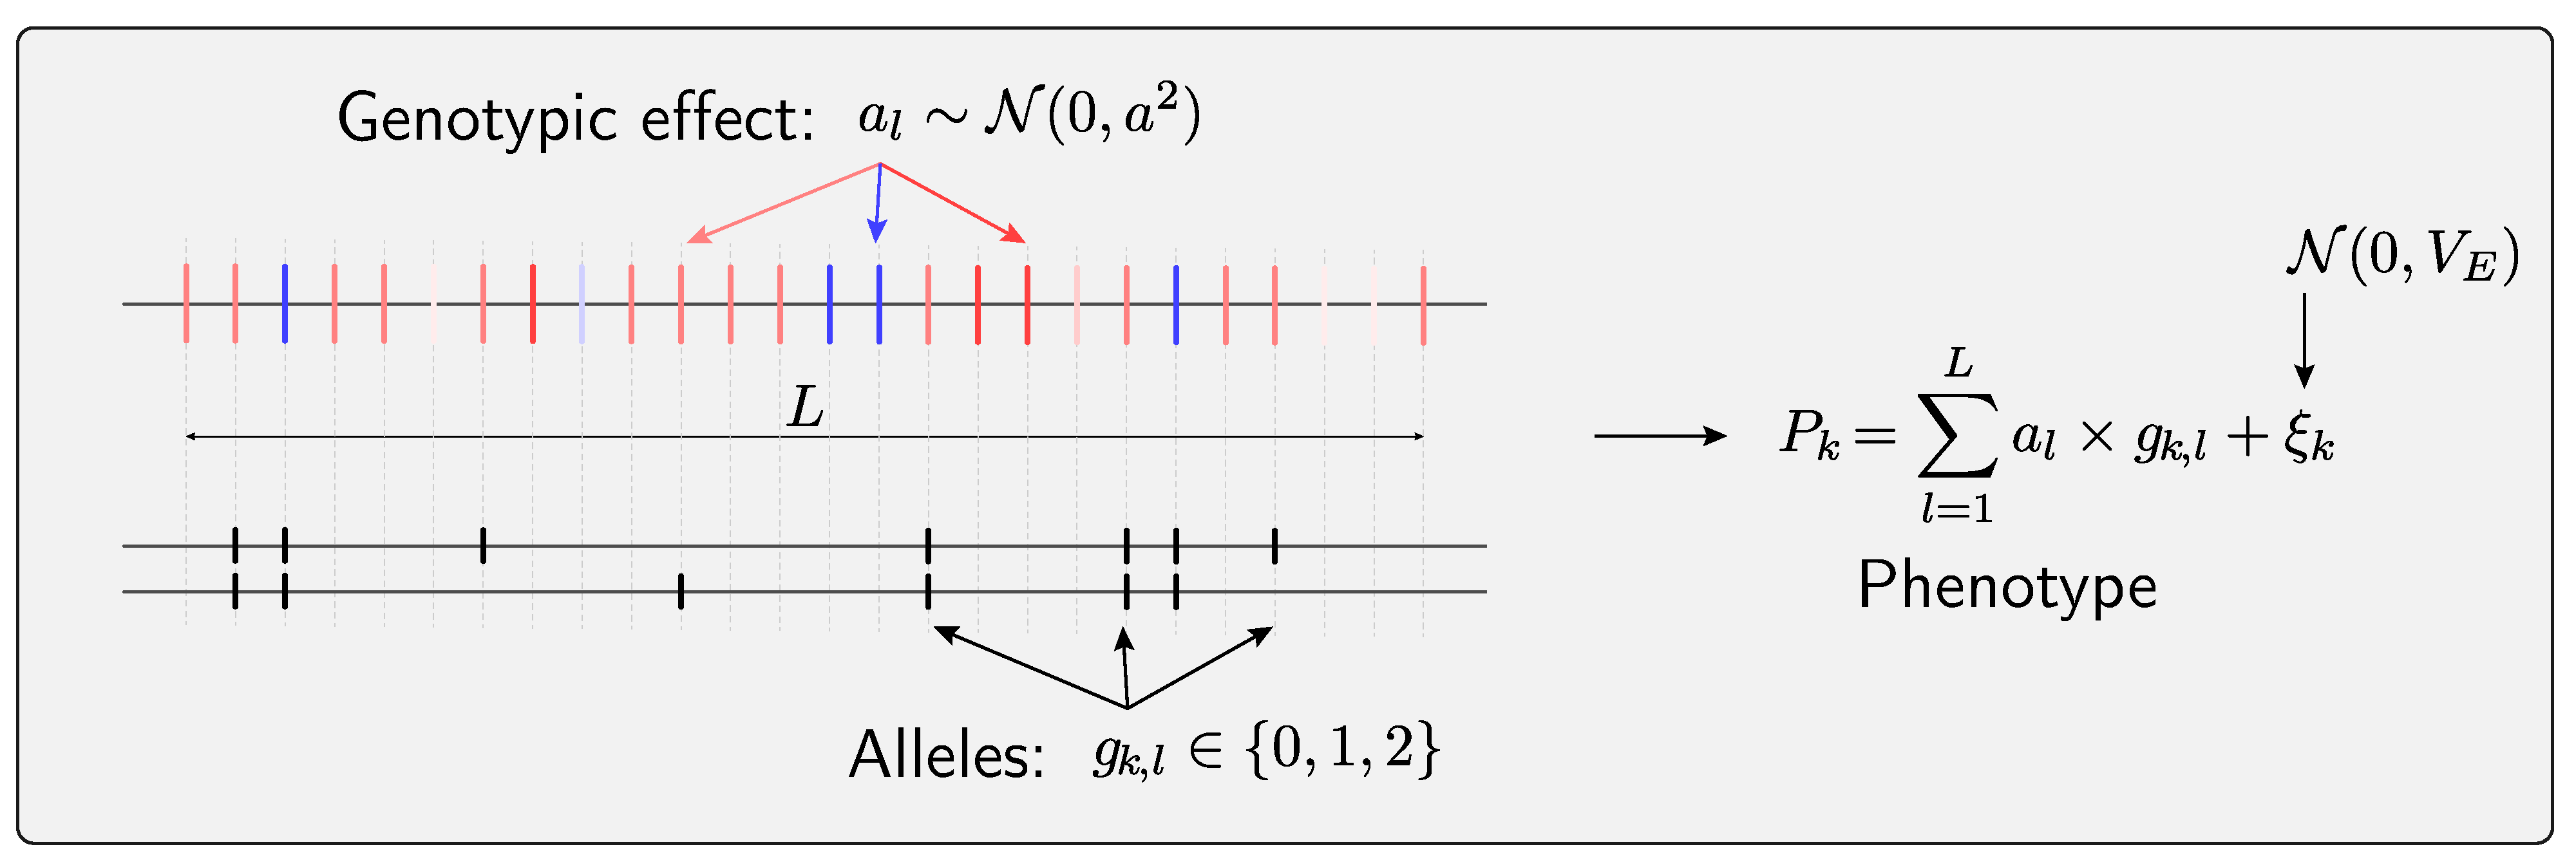
\includegraphics[width=0.6\textwidth, page=1] {figureS1}
    \label{fig:simulator-summary}
\end{center}

within-species, the mean ($\bar{G}$) and variance ($\VarGenetic$) of the genotype are:
\begin{equation}
    \bar{G} = \frac{1}{\Ne}\sum_{\Indiv=1}^{\Ne} G_{\Indiv} \text{\quad and \quad} \VarGenetic = \frac{1}{\Ne}\sum_{\Indiv=1}^{\Ne}\left(G_{\Indiv}- \bar{G} \right)^2\label{eq:simu-genotype}
\end{equation}
The theoretical additive genetic variance ($\VarGenetic$) is a function of the number of loci ($\NbrLoci$) and the effect of a mutation ($a$) as:
\begin{equation}
    \VarGenetic = 4 \Ne \Multiply \MutationRatePheno \Multiply \NbrLoci \Multiply a^2 \label{eq:simu-var-genetic}
\end{equation}

The mean ($\bar{\Trait}$) and variance ($\VarPhenotype$) of the phenotype are:
\begin{equation}
    \bar{\Trait} = \frac{1}{\Ne}\sum_{\Indiv=1}^{\Ne} \Trait_{\Indiv}\text{\quad and \quad} \VarPhenotype = \frac{1}{\Ne}\sum_{\Indiv=1}^{\Ne}\left(\Trait_{\Indiv} - \bar{\Trait} \right)^2 \label{eq:simu-between}
\end{equation}

Heritability ($\Heritability$) is defined as:
\begin{equation}
    \Heritability = \frac{\VarGenetic}{\VarPhenotype} = \frac{\VarGenetic}{\VarGenetic + \VarEnv}\label{eq:simu-heritability}
\end{equation}
Altogether, effective population size ($\Ne$), the number of loci ($\NbrLoci$) and the effect of a mutation ($a$), we can compute the variance of the environment ($\VarEnv$) that is required to reach a given heritability ($\Heritability$) as:
\begin{equation}
    \VarEnv = \VarGenetic \Multiply \left( \frac{1}{\Heritability} - 1 \right) = 4 \Ne \Multiply \MutationRatePheno \Multiply \NbrLoci \Multiply a^2 \Multiply \left( \frac{1}{\Heritability} - 1 \right) \label{eq:simu-var-env}
\end{equation}

\newpage
\section{Bayesian estimate}\label{sec:bayesian-estimate}

\subsection{Multivariate Brownian process}\label{subsec:multivariate-brownian-process}
Here we model $\Ntrait$ traits evolving along the phylogenetic tree that are correlated between them.
Their variation along the phylogeny is modeled as a $\Ntrait$-dimensional Brownian process $\Brownian$ ($1 \times \Ntrait$) starting at the root and branching along the tree topology.
The rate of change of the Brownian process is determined by the positive semi-definite and symmetric covariance matrix between traits $\CovarianceMatrix$ ($\Ntrait \times \Ntrait$).
Along branch $\Branch$ with length $d_{\Branch}$, the Brownian process start at the ancestral node $\mathcal{A}(\Branch)$ with value $\Brownian(\mathcal{A}(\Branch))$, and ends at node $\mathcal{R}(\Branch)$  with value $\Brownian(\mathcal{R}(\Branch))$.
The independent contrast $\contrast_{\Branch}$ defined as change in trait along the branch normalized by $\sqrt {d_{\Branch}}$ is a multivariate Gaussian:
\begin{equation}
    \label{eq:DistribBrownian}
    \contrast_{\Branch} = \frac{\Brownian (\mathcal{R}(\Branch)) - \Brownian (\mathcal{A}(\Branch)) }{\sqrt {d_{\Branch}}} \sim \mathcal{N}\left(\VecZero, \CovarianceMatrix \right).
\end{equation}

\subsection{Sampling the covariance matrix}\label{subsec:sampling-the-covariance-matrix}
From the independent contrast at each branch of the tree ($\contrast_{\Branch}$), we can define the $\Ntrait \times \Ntrait$ scatter matrix, $\Scattermatrix$, as:
\begin{equation}
    \Scattermatrix = \sum\limits_{\Branch=1}^{\Nbranch} \contrast_{\Branch} \MultiplyMatrix \contrast_{\Branch}\tr\label{eq:bayes-scatter},
\end{equation}
where $\Nbranch$ is the number of branches in the tree and $\NbrTaxa$ the number of taxa.

The {prior} on the covariance matrix is an inverse Wishart distribution, with $\Ntrait + 1$ degrees of freedom:
\begin{equation}
    \label{eq:Distribcovariance}
    \CovarianceMatrix \sim \text{Wishart}^{-1} (\Identitymatrix, \Ntrait + 1).
\end{equation}

By Bayes theorem, the {posterior} on $\CovarianceMatrix$, conditional on a particular realization of $\Brownian$ (and thus of $\contrast$) is an invert Wishart distribution, of parameter $\Identitymatrix + \Scattermatrix$ and with $\WishartPostDf$ degrees of freedom.
\begin{equation}
    \CovarianceMatrix \sim \text{Wishart}^{-1}\left( \Identitymatrix + \Scattermatrix, \WishartPostDf\right)\label{eq:bayes-posterior}
\end{equation}
This invert Wishart distribution can be obtained by sampling $\WishartPostDf$ independent and identically distributed multivariate normal random variables $\Multivariate_{\WishartIDD}$ defined by
\begin{equation}
    \Multivariate_{\WishartIDD} \sim \mathcal{N} \left( \VecZero, \left[ \Identitymatrix + \Scattermatrix\right]^{-1} \right).\label{eq:bayes-multivariate}
\end{equation}
And from these multivariate samples, $\CovarianceMatrix$ is Gibbs sampled as:
\begin{equation}
    \CovarianceMatrix = \left( \sum\limits_{\WishartIDD=1}^{\WishartPostDf} \Multivariate_{\WishartIDD} \MultiplyMatrix  \left[\Multivariate_{\WishartIDD} \right] \tr \right)\inv \label{eq:bayes-gibbs}
\end{equation}

\newpage
\section{Bayesian and Maximum-likelihood implementation}\label{sec:implementation}

Implementation is included within the \textit{BayesCode} software, available at \censor{\url{https://github.com/ThibaultLatrille/bayescode}}.

\subsection{Data formatting}\label{subsec:data-formatting}

Running the analysis on your dataset and compute posterior probabilities requires three files:
\begin{enumerate}
    \item A phylogenetic tree in newick format, with branch lengths in number of substitutions per site (neutral markers), from which the values of nucleotide divergence ($d$) used in denominator of eq.~\ref{eq:estimated-rate-phy} are used.
    \item A file containing the mean trait values for each species.
    \item A file containing the variation within-species for each trait and the genetic variation within-species (neutral markers).
\end{enumerate}

\subsubsection{Phylogenetic tree}

The phylogenetic tree must be in newick format, with branch lengths in substitutions per site (neutral markers).

\subsubsection{Mean trait for each species}

The file containing mean trait values for each species must be in a tab-delimited file with the following format:
\begin{center}
    \begin{adjustbox}{width = 0.35\textwidth}
        \begin{tabular}{|l|c|c|}
            \hline
            TaxonName            & Body\_mass & Brain\_mass \\
            \hline
            Panthera\_tigris     & 12.26      & 5.676       \\
            Pithecia\_pithecia   & 7.256      & 3.436       \\
            Colobus\_angolensis  & 9.176      & 4.284       \\
            Saimiri\_boliviensis & 6.845      & 3.279       \\
            $\vdots$             & $\vdots$   & $\vdots$    \\
            \hline
        \end{tabular}\label{tab:trait-mean}
    \end{adjustbox}
\end{center}

The columns are:
\begin{itemize}
    \item \emph{TaxonName}: the name of the taxon matching the name in the alignment and the tree.
    \item As many columns as traits, without spaces or special characters in the trait.
    \item The values can be \texttt{NaN} to indicate that the trait is not available for that taxon.
\end{itemize}

\newpage
\subsubsection{Trait variation for each species}

The file containing trait variation for each species must be in a tab-delimited file with the following format:
\begin{center}
    \begin{adjustbox}{width = 1.0\textwidth}
        \begin{tabular}{|l|c|c|c|c|c|c|}
            \hline
            TaxonName            & Nucleotide\_diversity & Body\_mass\_variance & Body\_mass\_heritability & Brain\_mass\_variance & Brain\_mass\_heritability \\
            \hline
            Pithecia\_pithecia   & 0.0016                & 0.22871              & 0.2                      & 0.00737               & 0.2                       \\
            Colobus\_angolensis  & 0.0017                & 0.00393              & 0.2                      & 0.00416               & 0.2                       \\
            Saimiri\_boliviensis & 0.0013                & 0.00022              & 0.2                      & 0.00045               & 0.2                       \\
            Pygathrix\_nemaeus   & 0.0016                & 0.00347              & 0.2                      & 0.00097               & 0.2                       \\
            $\vdots$             & $\vdots$              & $\vdots$             & $\vdots$                 & $\vdots$              & $\vdots$                  \\
            \hline
        \end{tabular}
        \label{tab:trait-variance}
    \end{adjustbox}
\end{center}

\begin{itemize}
    \item \emph{TaxonName}: the name of the taxon matching the name in the alignment and the tree.
    \item \emph{Nucleotide\_diversity}: the nucleotide diversity within-species (neutral markers), cannot be \texttt{NaN}.
    \item As many columns as traits, without spaces or special characters in the trait.
    \item \emph{TraitName\_variance}: the phenotypic variance of the trait within-species, can be \texttt{NaN} to indicate that the trait variance is not available for that taxon.
    \item \emph{TraitName\_heritability} (optional): the heritability of the trait within-species, between 0 and 1, cannot be \texttt{NaN}.
    \item The columns with the suffix \texttt{\_variance} and \texttt{\_heritability} are repeated for each trait.
    \item \emph{TraitName\_heritability\_lower} (optional): the lower bound of the heritability of the trait within-species, between 0 and 1, cannot be \texttt{NaN}.
    \item \emph{TraitName\_heritability\_upper} (optional): the upper bound of the heritability of the trait within-species, between 0 and 1, cannot be \texttt{NaN}.
    \item If the columns with the suffix \texttt{\_heritability\_lower} and \texttt{\_heritability\_upper} are present, the heritability is randomly drawn from a uniform distribution between the lower and upper bounds.
    \item If the columns with the suffix \texttt{\_heritability} is present, it is taken as is.
    \item If the additive genetic variance (instead of phenotypic variance) is available for a trait, the heritability can be omitted and will automatically be set to 1.0.
\end{itemize}

\newpage
\subsection{Bayesian estimation}\label{subsec:running-nodetraitsand-readnodetraits}

The executable \texttt{nodetraits} from \textit{BayesCode} is used to run the Bayesian estimation of the model, and the executable \texttt{readnodetraits} is used to read the results.

Assuming that the file \texttt{data/body\_size/mammals.male.tsv} contains the mean trait values for each species, the file \texttt{data/body\_size/mammals.male.var\_trait.tsv} contains the variation within-species for each trait and the genetic variation within-species (neutral markers), and the file \texttt{data/body\_size/mammals.male.tree} contains the phylogenetic tree, the following commands are used to run the model and read the results.

\subsubsection{Running the model}
\texttt{nodetraits} is run with the following command:
\begin{lstlisting}[language = sh,label={lst:nodetraits-run}]
nodetraits  --until 2000
            --tree data/body_size/mammals.male.tree
            --traitsfile data/body_size/mammals.male.tsv
            run_mammals_male
\end{lstlisting}

\subsubsection{Reading the results}
Once the model has run, the chain \texttt{run\_mammals\_male} is used to compute the posterior distribution of the ratio of between-species variation over within-species variation with \texttt{readnodetraits}:
\begin{lstlisting}[language = sh,label={lst:readnodetraits-rho}]
readnodetraits --burnin 1000
               --var_within data/body_size/mammals.male.var_trait.tsv
               --output results_mammals_male.tsv
               run_mammals_male
\end{lstlisting}
The file \texttt{data\_empirical/chain\_name.ratio.tsv} then contains the posterior mean of the ratio of between-species variation over within-species variation, the 95\% and 99\% credible interval, and the posterior probability that the ratio is greater than 1.

\subsection{Maximum likelihood estimation}\label{subsec:maximum-likelihood-estimation}

To obtain the ratio (without the posterior credible interval and probability) using maximum likelihood computation, the following python script can be used:
\begin{lstlisting}[language = sh, label={lst:neutrality_index}]
python3 utils/neutrality_index.py --tree data/body_size/mammals.male.tree
                                  --traitsfile data/body_size/mammals.male.tsv
                                  --var_within data/body_size/mammals.male.var_trait.tsv
                                  --output results_ML_mammals_male.tsv
\end{lstlisting}

\newpage
\section{Saturation of phenotypic divergence}\label{sec:supp-distance}

\DIFdelbegin \DIFdel{The phenotype is encoded by a genetic architecture and is thus ultimately bounded.
At the macro-evolutionary scale, phenotypic divergence should plateau at some point}\DIFdelend \DIFaddbegin \DIFadd{In our simulation setting, the genetic architecture underlying the phenotype is not changing along the phylogeny.
As a result, the phenotype may be bounded by what such genetic architecture can produce, and this could cause a slowdown of phenotypic divergence over time}\DIFaddend , ultimately resulting in a \DIFaddbegin \DIFadd{decreased }\DIFaddend $\RateBetween$.

\begin{center}
    \captionof{figure}{Saturation of phenotypic divergence.}
    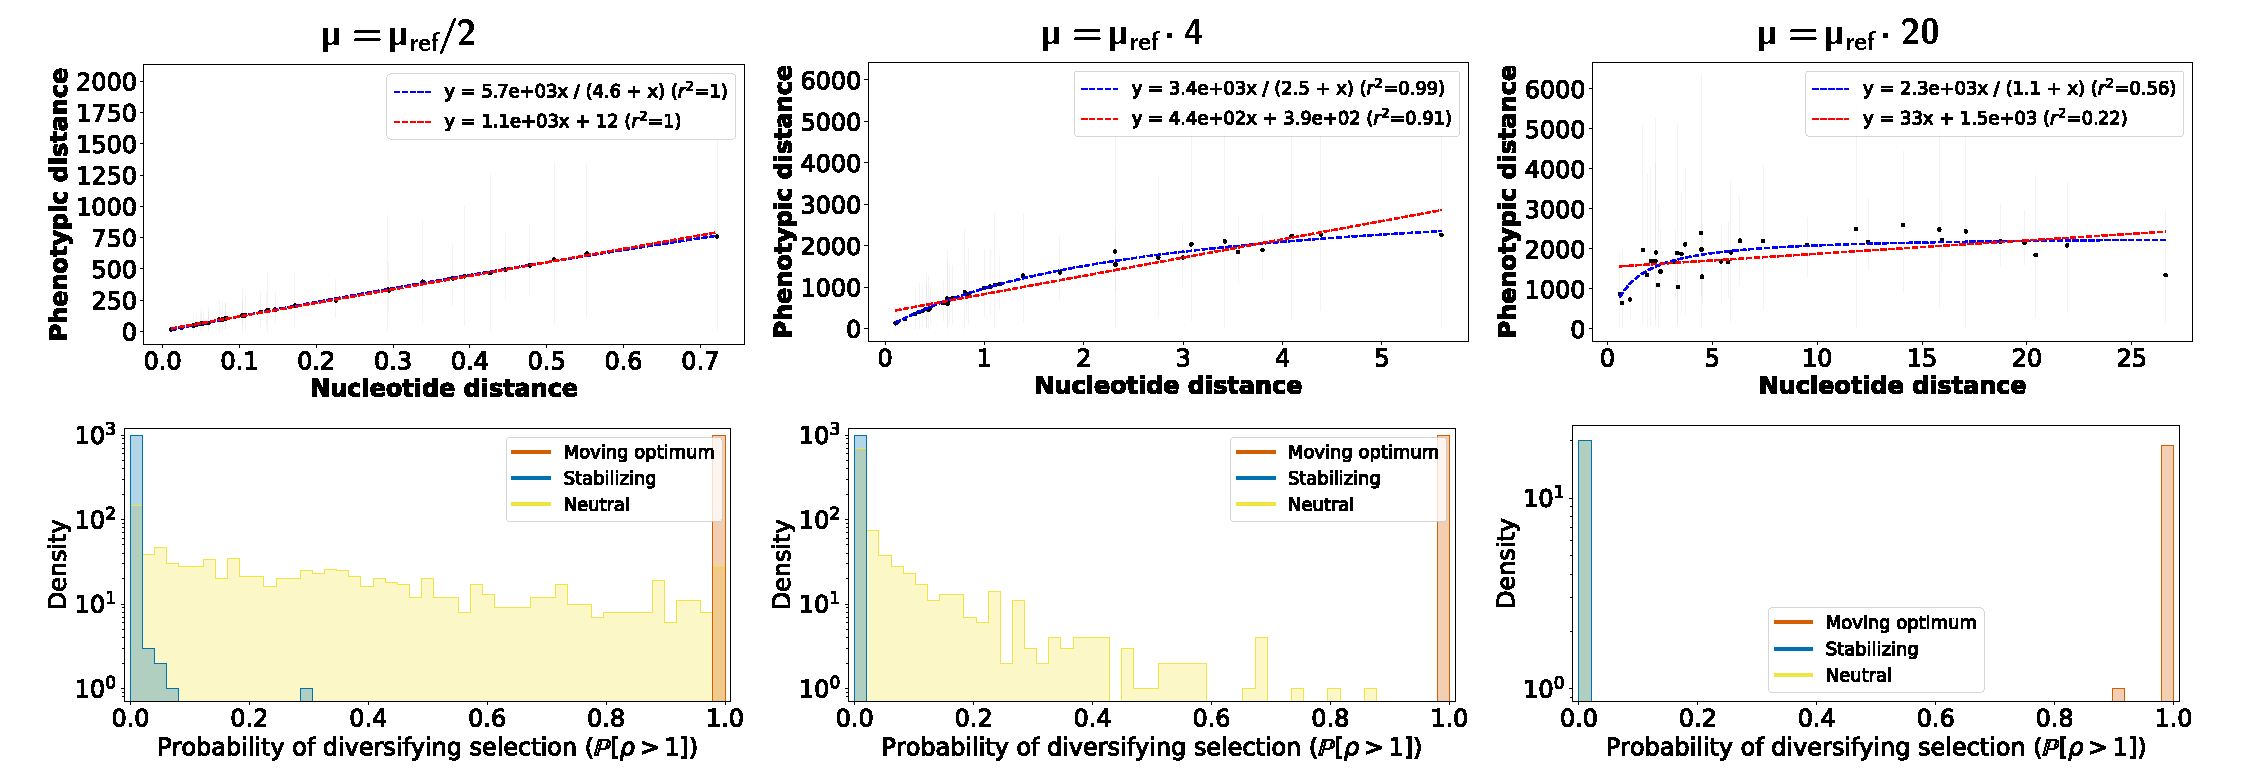
\includegraphics[width=1.0\textwidth, page=1] {figureS2}
    \label{fig:supp-distance}
\end{center}
\begin{itemize}
    \item Left column: $1,000$ simulations with low divergence between species (half that of mammals).
    \item Middle column: $1,000$ simulations with high divergence between species (4 times that of mammals).
    \item Right column: $200$ simulations with very high divergence between species (20 times that of mammals).
    \item Top row: Simulation of neutral trait, phenotypic divergence between species as a function of the nucleotide divergence. Phenotypic divergence is computed between two species as the covariance between the trait ($\VarPhy$), and the nucleotide divergence is computed as the number of substitutions per site shared between the two species ($d$). Each point is a pair of species, and the bounds of the intervals in grey are the 2.5\% and 97.5\% quantiles across the replicates. The blue line is the linear regression and the red line is the saturation model ($y = \alpha \Multiply x / (\beta + x)$).
    \item Bottom row: Traits simulated under stabilizing selection (blue), under a neutral evolution (yellow), and under a moving optimum (red). Histogram of probabilities of \DIFdelbegin \DIFdel{$\EstNI$ }\DIFdelend \DIFaddbegin \DIFadd{$\NI$ }\DIFaddend being greater than $1$.
\end{itemize}
Under a model of neutral trait evolution, when mutation rate increases, or equivalently the divergence between species increases, the phenotypic divergence between species saturates faster than the nucleotide divergence.
This saturation effect can result in a spurious signal of stabilizing selection (\DIFdelbegin \DIFdel{$\EstNI < 1$}\DIFdelend \DIFaddbegin \DIFadd{$\NI < 1$}\DIFaddend ) for deeper phylogeny when the trait is evolving neutrally.
\end{document}
%TC:endignore